% Options for packages loaded elsewhere
\PassOptionsToPackage{unicode}{hyperref}
\PassOptionsToPackage{hyphens}{url}
\documentclass[
]{book}
\usepackage{xcolor}
\usepackage{amsmath,amssymb}
\setcounter{secnumdepth}{5}
\usepackage{iftex}
\ifPDFTeX
  \usepackage[T1]{fontenc}
  \usepackage[utf8]{inputenc}
  \usepackage{textcomp} % provide euro and other symbols
\else % if luatex or xetex
  \usepackage{unicode-math} % this also loads fontspec
  \defaultfontfeatures{Scale=MatchLowercase}
  \defaultfontfeatures[\rmfamily]{Ligatures=TeX,Scale=1}
\fi
\usepackage{lmodern}
\ifPDFTeX\else
  % xetex/luatex font selection
\fi
% Use upquote if available, for straight quotes in verbatim environments
\IfFileExists{upquote.sty}{\usepackage{upquote}}{}
\IfFileExists{microtype.sty}{% use microtype if available
  \usepackage[]{microtype}
  \UseMicrotypeSet[protrusion]{basicmath} % disable protrusion for tt fonts
}{}
\makeatletter
\@ifundefined{KOMAClassName}{% if non-KOMA class
  \IfFileExists{parskip.sty}{%
    \usepackage{parskip}
  }{% else
    \setlength{\parindent}{0pt}
    \setlength{\parskip}{6pt plus 2pt minus 1pt}}
}{% if KOMA class
  \KOMAoptions{parskip=half}}
\makeatother
\usepackage{color}
\usepackage{fancyvrb}
\newcommand{\VerbBar}{|}
\newcommand{\VERB}{\Verb[commandchars=\\\{\}]}
\DefineVerbatimEnvironment{Highlighting}{Verbatim}{commandchars=\\\{\}}
% Add ',fontsize=\small' for more characters per line
\usepackage{framed}
\definecolor{shadecolor}{RGB}{248,248,248}
\newenvironment{Shaded}{\begin{snugshade}}{\end{snugshade}}
\newcommand{\AlertTok}[1]{\textcolor[rgb]{0.94,0.16,0.16}{#1}}
\newcommand{\AnnotationTok}[1]{\textcolor[rgb]{0.56,0.35,0.01}{\textbf{\textit{#1}}}}
\newcommand{\AttributeTok}[1]{\textcolor[rgb]{0.13,0.29,0.53}{#1}}
\newcommand{\BaseNTok}[1]{\textcolor[rgb]{0.00,0.00,0.81}{#1}}
\newcommand{\BuiltInTok}[1]{#1}
\newcommand{\CharTok}[1]{\textcolor[rgb]{0.31,0.60,0.02}{#1}}
\newcommand{\CommentTok}[1]{\textcolor[rgb]{0.56,0.35,0.01}{\textit{#1}}}
\newcommand{\CommentVarTok}[1]{\textcolor[rgb]{0.56,0.35,0.01}{\textbf{\textit{#1}}}}
\newcommand{\ConstantTok}[1]{\textcolor[rgb]{0.56,0.35,0.01}{#1}}
\newcommand{\ControlFlowTok}[1]{\textcolor[rgb]{0.13,0.29,0.53}{\textbf{#1}}}
\newcommand{\DataTypeTok}[1]{\textcolor[rgb]{0.13,0.29,0.53}{#1}}
\newcommand{\DecValTok}[1]{\textcolor[rgb]{0.00,0.00,0.81}{#1}}
\newcommand{\DocumentationTok}[1]{\textcolor[rgb]{0.56,0.35,0.01}{\textbf{\textit{#1}}}}
\newcommand{\ErrorTok}[1]{\textcolor[rgb]{0.64,0.00,0.00}{\textbf{#1}}}
\newcommand{\ExtensionTok}[1]{#1}
\newcommand{\FloatTok}[1]{\textcolor[rgb]{0.00,0.00,0.81}{#1}}
\newcommand{\FunctionTok}[1]{\textcolor[rgb]{0.13,0.29,0.53}{\textbf{#1}}}
\newcommand{\ImportTok}[1]{#1}
\newcommand{\InformationTok}[1]{\textcolor[rgb]{0.56,0.35,0.01}{\textbf{\textit{#1}}}}
\newcommand{\KeywordTok}[1]{\textcolor[rgb]{0.13,0.29,0.53}{\textbf{#1}}}
\newcommand{\NormalTok}[1]{#1}
\newcommand{\OperatorTok}[1]{\textcolor[rgb]{0.81,0.36,0.00}{\textbf{#1}}}
\newcommand{\OtherTok}[1]{\textcolor[rgb]{0.56,0.35,0.01}{#1}}
\newcommand{\PreprocessorTok}[1]{\textcolor[rgb]{0.56,0.35,0.01}{\textit{#1}}}
\newcommand{\RegionMarkerTok}[1]{#1}
\newcommand{\SpecialCharTok}[1]{\textcolor[rgb]{0.81,0.36,0.00}{\textbf{#1}}}
\newcommand{\SpecialStringTok}[1]{\textcolor[rgb]{0.31,0.60,0.02}{#1}}
\newcommand{\StringTok}[1]{\textcolor[rgb]{0.31,0.60,0.02}{#1}}
\newcommand{\VariableTok}[1]{\textcolor[rgb]{0.00,0.00,0.00}{#1}}
\newcommand{\VerbatimStringTok}[1]{\textcolor[rgb]{0.31,0.60,0.02}{#1}}
\newcommand{\WarningTok}[1]{\textcolor[rgb]{0.56,0.35,0.01}{\textbf{\textit{#1}}}}
\usepackage{longtable,booktabs,array}
\usepackage{calc} % for calculating minipage widths
% Correct order of tables after \paragraph or \subparagraph
\usepackage{etoolbox}
\makeatletter
\patchcmd\longtable{\par}{\if@noskipsec\mbox{}\fi\par}{}{}
\makeatother
% Allow footnotes in longtable head/foot
\IfFileExists{footnotehyper.sty}{\usepackage{footnotehyper}}{\usepackage{footnote}}
\makesavenoteenv{longtable}
\usepackage{graphicx}
\makeatletter
\newsavebox\pandoc@box
\newcommand*\pandocbounded[1]{% scales image to fit in text height/width
  \sbox\pandoc@box{#1}%
  \Gscale@div\@tempa{\textheight}{\dimexpr\ht\pandoc@box+\dp\pandoc@box\relax}%
  \Gscale@div\@tempb{\linewidth}{\wd\pandoc@box}%
  \ifdim\@tempb\p@<\@tempa\p@\let\@tempa\@tempb\fi% select the smaller of both
  \ifdim\@tempa\p@<\p@\scalebox{\@tempa}{\usebox\pandoc@box}%
  \else\usebox{\pandoc@box}%
  \fi%
}
% Set default figure placement to htbp
\def\fps@figure{htbp}
\makeatother
\setlength{\emergencystretch}{3em} % prevent overfull lines
\providecommand{\tightlist}{%
  \setlength{\itemsep}{0pt}\setlength{\parskip}{0pt}}
\usepackage[]{natbib}
\bibliographystyle{plainnat}
\usepackage{booktabs}
\usepackage{bookmark}
\IfFileExists{xurl.sty}{\usepackage{xurl}}{} % add URL line breaks if available
\urlstyle{same}
\hypersetup{
  pdftitle={Week 2: Reading, Exporting, and Checking Data},
  pdfauthor={Samuel Rowe},
  hidelinks,
  pdfcreator={LaTeX via pandoc}}

\title{Week 2: Reading, Exporting, and Checking Data}
\author{Samuel Rowe}
\date{2025-09-10}

\begin{document}
\maketitle

{
\setcounter{tocdepth}{1}
\tableofcontents
}
\chapter{Overview}\label{overview}

We will cover importing and exporting data. Some of this may be a review, but there are helpful options that you may have missed. We will also cover ways to check for data quality issues. This will be an important session, especially considering measurement error is a potential source of bias.

\emph{Note: }Recommended resources
UCLA OARC Stata resources: \url{https://stats.oarc.ucla.edu/stata/modules/}

I have used this source on numerous times. Even when you become proficient with Stata, UCLA's OARC Stata resources have been very helpful. If you just type \emph{UCLA OARC Stata } in a search engine, then it will usually pop up.

Statalist if usually another good resource when trying to figure out what went wrong. If you ask as question on the listserve, you will likely be scolded by Nick Cox, or you will be told to ``read the manual''. However, if you just read what others have asked, you will often find useful information.

Overview:
- Importing Data
- Exporting Data
- Data Checks and Cleaning

\chapter{Ingesting Data}\label{ingesting-data}

\emph{Mitchell Chapter 2}

Note when your working directory, I recommend using ``/'' instead of ``"
Stata will use both, and the backslash''\," often runs into string issues.

\section{Getting our data}\label{getting-our-data}

We'll get our data that we will use for the course.

\begin{Shaded}
\begin{Highlighting}[]
\NormalTok{pwd}
\NormalTok{*Set your working directory}
\NormalTok{cd }\StringTok{"/Users/Sam/Desktop/Econ 645/Data/"}

\NormalTok{*Use:}
\NormalTok{net from https:}\CommentTok{//www.stata{-}press.com/data/dmus2}
\NormalTok{net }\FunctionTok{get}\NormalTok{ dmus1}
\NormalTok{net }\FunctionTok{get}\NormalTok{ dmus2}

\NormalTok{*All commands:}
\NormalTok{net install dmus1}
\end{Highlighting}
\end{Shaded}

\section{Reading Stata data}\label{reading-stata-data}

We use the \emph{use} command to read Stata data. Use the clear option to clear the data from memory so you can read the data file. Otherwise, you will get an error

We'll add the clear option to clear our memory to provide an error

\begin{Shaded}
\begin{Highlighting}[]
\NormalTok{cd }\StringTok{"/Users/Sam/Desktop/Econ 645/Data/Mitchell/"}
\KeywordTok{use} \StringTok{"dentists.dta"}\NormalTok{, }\KeywordTok{clear}
\OtherTok{list}  
\end{Highlighting}
\end{Shaded}

\begin{verbatim}
/Users/Sam/Desktop/Econ 645/Data/Mitchell

     +----------------------------------------------+
     |              name   years   fulltime   recom |
     |----------------------------------------------|
  1. | Y. Don Uflossmore    7.25          0       1 |
  2. |    Olive Tu'Drill   10.25          1       1 |
  3. | Isaac O'Yerbreath   32.75          1       1 |
  4. |      Ruth Canaale      22          1       1 |
  5. |        Mike Avity     8.5          0       0 |
     +----------------------------------------------+
\end{verbatim}

We can read Stata data from websources. From Stata Press website:

\begin{Shaded}
\begin{Highlighting}[]
\KeywordTok{use} \StringTok{"https://www.stata{-}press.com/data/dmus2/dentists.dta"}\NormalTok{, }\KeywordTok{clear}
\OtherTok{list}
\end{Highlighting}
\end{Shaded}

\begin{verbatim}
     |              name   years   fulltime   recom |
     |----------------------------------------------|
  1. | Y. Don Uflossmore    7.25          0       1 |
  2. |    Olive Tu'Drill   10.25          1       1 |
  3. | Isaac O'Yerbreath   32.75          1       1 |
  4. |      Ruth Canaale      22          1       1 |
  5. |        Mike Avity     8.5          0       0 |
     +----------------------------------------------+
\end{verbatim}

From NBER website

\begin{Shaded}
\begin{Highlighting}[]
\KeywordTok{use} \StringTok{"https://data.nber.org/morg/annual/morg20.dta"}\NormalTok{, }\KeywordTok{clear}
\OtherTok{list}\NormalTok{ lfsr94 stfips sex }\KeywordTok{in}\NormalTok{ f/10}
\end{Highlighting}
\end{Shaded}

\begin{verbatim}
     |                      lfsr94   stfips   sex |
     |--------------------------------------------|
  1. |            Employed-At Work       AL     2 |
  2. |            Employed-At Work       AL     1 |
  3. |  Retired-Not In Labor Force       AL     1 |
  4. |  Retired-Not In Labor Force       AL     2 |
  5. |    Other-Not In Labor Force       AL     2 |
     |--------------------------------------------|
  6. | Disabled-Not In Labor Force       AL     1 |
  7. |  Retired-Not In Labor Force       AL     1 |
  8. |  Retired-Not In Labor Force       AL     2 |
  9. |  Retired-Not In Labor Force       AL     2 |
 10. |  Retired-Not In Labor Force       AL     1 |
     +--------------------------------------------+
\end{verbatim}

\section{Reading Stata data with subsets}\label{reading-stata-data-with-subsets}

Subsetting can be a helpful method to read in extremely large data sets, such as American Community Survey (ACS) public use file. We can subset by variables, observations, or both.

\subsection{Subsetting by columns (variables)}\label{subsetting-by-columns-variables}

You can read in a subset of Stata data by columns. This can be helpful when you have a large dataset but only need a few columns of data. However, you need to know the variable names. We will need to have a data dictionary in order to do this. The January CPS data dictionary can be found on Census's website. \url{https://www2.census.gov/programs-surveys/cps/datasets/2025/basic/2025_Basic_CPS_Public_Use_Record_Layout_plus_IO_Code_list.txt}

\begin{Shaded}
\begin{Highlighting}[]
\KeywordTok{quietly}\NormalTok{ cd }\StringTok{"/Users/Sam/Desktop/Data/CPS/"}
\KeywordTok{use}\NormalTok{ gestfips pemlr pternwa }\KeywordTok{using} \StringTok{"smalljul25pub.dta"}\NormalTok{, }\KeywordTok{clear}
\OtherTok{list} \KeywordTok{in}\NormalTok{ 1/3}
\end{Highlighting}
\end{Shaded}

\begin{verbatim}
     | gestfips   pemlr   pternwa |
     |----------------------------|
  1. |        1       .         . |
  2. |        1       5        -1 |
  3. |        1       6        -1 |
     +----------------------------+
\end{verbatim}

If it is a large dataset, I don't recommend using list by itself. Use in \emph{1/N}

\subsection{Subsetting by rows (observations)}\label{subsetting-by-rows-observations}

You can read in a subset of data by rows. In my opinion, this is a better method to subset than by columns. You are able to see the entire dataset. You can use a qualifiers \emph{if} or \emph{in}

\begin{Shaded}
\begin{Highlighting}[]
\KeywordTok{quietly}\NormalTok{ cd }\StringTok{"/Users/Sam/Desktop/Data/CPS/"}
\KeywordTok{use} \StringTok{"smalljul25pub.dta"} \KeywordTok{if}\NormalTok{ gestfip == 24 \& prtage == 30, }\KeywordTok{clear}
\OtherTok{list} \KeywordTok{in}\NormalTok{ 1/10}
\end{Highlighting}
\end{Shaded}

\begin{verbatim}
  1. | hrhhid2 | hrmis | hrmonth | hryear4 | gestfips | gediv | pulineno | pudis | puiodp1 | puiodp2 | puiodp3  |
     |   17011 |     7 |       7 |    2025 |       24 |     5 |        3 |    -1 |      -1 |      -1 |      -1  |
     |-------------------------------------+----------+---------------------------------------------------------|
     | perrp | pesex | pemaritl | pehspnon | peeduca  | peafever  | ptdtrace  | prpertyp  | prtage  | pehractt  |
     |    49 |     1 |        6 |        2 |      40  |        2  |        2  |        2  |     30  |       12  |
     |------------------------------------------------------------------------------------+---------------------|
     | pehract1 | pehract2 | pemlr | peio1icd | peio1cow | peio2cow | prmjind1 | prmjind2 | prmjocc1 | prmjocc2 |
     |       12 |       -1 |     1 |     6380 |        4 |       -1 |        6 |       -1 |        5 |       -1 |
     |----------+----------+-------------------------------------------------------------------------+----------|
     | prdtind1 | prdtind2 | prdtocc1 | prdtocc2 | prsjmj | peernhry | peernhro | peernlab | prerelg | prdisflg |
     |       23 |       -1 |       17 |       -1 |      1 |       -1 |       -1 |       -1 |       0 |        2 |
     |----------+----------+----------+-------------------------------------------------------------------------|
     | pecert1  | pecert2  | pecert3  |  pwcmpwgt  |  pternwa  |  ptio1ocd  |     hrhhid  |  ptwk  |  gtmetsta  |
     |       2  |      -1  |      -1  |  99149562  |       -1  |      5510  |  9.401e+14  |     0  |         1  |
     +----------------------------------------------------------------------------------------------------------+

     +----------------------------------------------------------------------------------------------------------+
  2. | hrhhid2 | hrmis | hrmonth | hryear4 | gestfips | gediv | pulineno | pudis | puiodp1 | puiodp2 | puiodp3  |
     |   17011 |     6 |       7 |    2025 |       24 |     5 |        2 |    -1 |       1 |       2 |       1  |
     |-------------------------------------+----------+---------------------------------------------------------|
     | perrp | pesex | pemaritl | pehspnon | peeduca  | peafever  | ptdtrace  | prpertyp  | prtage  | pehractt  |
     |    51 |     1 |        1 |        2 |      39  |        2  |        4  |        2  |     30  |       52  |
     |------------------------------------------------------------------------------------+---------------------|
     | pehract1 | pehract2 | pemlr | peio1icd | peio1cow | peio2cow | prmjind1 | prmjind2 | prmjocc1 | prmjocc2 |
     |       44 |        8 |     1 |      770 |        4 |       -1 |        3 |       -1 |        8 |       -1 |
     |----------+----------+-------------------------------------------------------------------------+----------|
     | prdtind1 | prdtind2 | prdtocc1 | prdtocc2 | prsjmj | peernhry | peernhro | peernlab | prerelg | prdisflg |
     |        4 |       -1 |       20 |       -1 |      2 |       -1 |       -1 |       -1 |       0 |        2 |
     |----------+----------+----------+-------------------------------------------------------------------------|
     | pecert1  | pecert2  | pecert3  |  pwcmpwgt  |  pternwa  |  ptio1ocd  |     hrhhid  |  ptwk  |  gtmetsta  |
     |       2  |      -1  |      -1  |  48285071  |       -1  |      7315  |  4.700e+13  |     0  |         1  |
     +----------------------------------------------------------------------------------------------------------+

     +----------------------------------------------------------------------------------------------------------+
  3. | hrhhid2 | hrmis | hrmonth | hryear4 | gestfips | gediv | pulineno | pudis | puiodp1 | puiodp2 | puiodp3  |
     |   17012 |     8 |       7 |    2025 |       24 |     5 |        1 |    -1 |       1 |       2 |       1  |
     |-------------------------------------+----------+---------------------------------------------------------|
     | perrp | pesex | pemaritl | pehspnon | peeduca  | peafever  | ptdtrace  | prpertyp  | prtage  | pehractt  |
     |    41 |     1 |        6 |        2 |      42  |        2  |        2  |        2  |     30  |       40  |
     |------------------------------------------------------------------------------------+---------------------|
     | pehract1 | pehract2 | pemlr | peio1icd | peio1cow | peio2cow | prmjind1 | prmjind2 | prmjocc1 | prmjocc2 |
     |       40 |       -1 |     1 |     7280 |        4 |       -1 |        9 |       -1 |        5 |       -1 |
     |----------+----------+-------------------------------------------------------------------------+----------|
     | prdtind1 | prdtind2 | prdtocc1 | prdtocc2 | prsjmj | peernhry | peernhro | peernlab | prerelg | prdisflg |
     |       36 |       -1 |       17 |       -1 |      1 |        2 |       -1 |        2 |       1 |        2 |
     |----------+----------+----------+-------------------------------------------------------------------------|
     | pecert1  | pecert2  | pecert3  |  pwcmpwgt  |  pternwa  |  ptio1ocd  |     hrhhid  |  ptwk  |  gtmetsta  |
     |       2  |      -1  |      -1  | 113138434  |   183000  |      5120  |  3.411e+14  |     0  |         1  |
     +----------------------------------------------------------------------------------------------------------+

     +----------------------------------------------------------------------------------------------------------+
  4. | hrhhid2 | hrmis | hrmonth | hryear4 | gestfips | gediv | pulineno | pudis | puiodp1 | puiodp2 | puiodp3  |
     |   19011 |     3 |       7 |    2025 |       24 |     5 |        4 |    -1 |      -1 |      -1 |      -1  |
     |-------------------------------------+----------+---------------------------------------------------------|
     | perrp | pesex | pemaritl | pehspnon | peeduca  | peafever  | ptdtrace  | prpertyp  | prtage  | pehractt  |
     |    49 |     1 |        6 |        2 |      39  |        2  |        1  |        2  |     30  |       32  |
     |------------------------------------------------------------------------------------+---------------------|
     | pehract1 | pehract2 | pemlr | peio1icd | peio1cow | peio2cow | prmjind1 | prmjind2 | prmjocc1 | prmjocc2 |
     |       32 |       -1 |     1 |      770 |        4 |       -1 |        3 |       -1 |       10 |       -1 |
     |----------+----------+-------------------------------------------------------------------------+----------|
     | prdtind1 | prdtind2 | prdtocc1 | prdtocc2 | prsjmj | peernhry | peernhro | peernlab | prerelg | prdisflg |
     |        4 |       -1 |       22 |       -1 |      1 |       -1 |       -1 |       -1 |       0 |        2 |
     |----------+----------+----------+-------------------------------------------------------------------------|
     | pecert1  | pecert2  | pecert3  |  pwcmpwgt  |  pternwa  |  ptio1ocd  |     hrhhid  |  ptwk  |  gtmetsta  |
     |       2  |      -1  |      -1  |  44333596  |       -1  |      9130  |  9.007e+14  |     0  |         1  |
     +----------------------------------------------------------------------------------------------------------+

     +----------------------------------------------------------------------------------------------------------+
  5. | hrhhid2 | hrmis | hrmonth | hryear4 | gestfips | gediv | pulineno | pudis | puiodp1 | puiodp2 | puiodp3  |
     |   19011 |     2 |       7 |    2025 |       24 |     5 |        1 |    -1 |       1 |       2 |       1  |
     |-------------------------------------+----------+---------------------------------------------------------|
     | perrp | pesex | pemaritl | pehspnon | peeduca  | peafever  | ptdtrace  | prpertyp  | prtage  | pehractt  |
     |    40 |     1 |        1 |        2 |      39  |        2  |        1  |        2  |     30  |       50  |
     |------------------------------------------------------------------------------------+---------------------|
     | pehract1 | pehract2 | pemlr | peio1icd | peio1cow | peio2cow | prmjind1 | prmjind2 | prmjocc1 | prmjocc2 |
     |       50 |       -1 |     1 |      170 |        4 |       -1 |        1 |       -1 |        6 |       -1 |
     |----------+----------+-------------------------------------------------------------------------+----------|
     | prdtind1 | prdtind2 | prdtocc1 | prdtocc2 | prsjmj | peernhry | peernhro | peernlab | prerelg | prdisflg |
     |        1 |       -1 |       18 |       -1 |      1 |       -1 |       -1 |       -1 |       0 |        2 |
     |----------+----------+----------+-------------------------------------------------------------------------|
     | pecert1  | pecert2  | pecert3  |  pwcmpwgt  |  pternwa  |  ptio1ocd  |     hrhhid  |  ptwk  |  gtmetsta  |
     |       2  |      -1  |      -1  |  31435370  |       -1  |      6050  |  9.450e+14  |     0  |         1  |
     +----------------------------------------------------------------------------------------------------------+

     +----------------------------------------------------------------------------------------------------------+
  6. | hrhhid2 | hrmis | hrmonth | hryear4 | gestfips | gediv | pulineno | pudis | puiodp1 | puiodp2 | puiodp3  |
     |   17011 |     5 |       7 |    2025 |       24 |     5 |        1 |    -1 |      -1 |      -1 |      -1  |
     |-------------------------------------+----------+---------------------------------------------------------|
     | perrp | pesex | pemaritl | pehspnon | peeduca  | peafever  | ptdtrace  | prpertyp  | prtage  | pehractt  |
     |    41 |     1 |        6 |        1 |      45  |        2  |        4  |        2  |     30  |       40  |
     |------------------------------------------------------------------------------------+---------------------|
     | pehract1 | pehract2 | pemlr | peio1icd | peio1cow | peio2cow | prmjind1 | prmjind2 | prmjocc1 | prmjocc2 |
     |       40 |       -1 |     1 |     7980 |        4 |       -1 |       10 |       -1 |        2 |       -1 |
     |----------+----------+-------------------------------------------------------------------------+----------|
     | prdtind1 | prdtind2 | prdtocc1 | prdtocc2 | prsjmj | peernhry | peernhro | peernlab | prerelg | prdisflg |
     |       42 |       -1 |       10 |       -1 |      1 |       -1 |       -1 |       -1 |       0 |        2 |
     |----------+----------+----------+-------------------------------------------------------------------------|
     | pecert1  | pecert2  | pecert3  |  pwcmpwgt  |  pternwa  |  ptio1ocd  |     hrhhid  |  ptwk  |  gtmetsta  |
     |       1  |       1  |       1  |  75007444  |       -1  |      3010  |  4.260e+14  |     0  |         1  |
     +----------------------------------------------------------------------------------------------------------+

     +----------------------------------------------------------------------------------------------------------+
  7. | hrhhid2 | hrmis | hrmonth | hryear4 | gestfips | gediv | pulineno | pudis | puiodp1 | puiodp2 | puiodp3  |
     |   19011 |     3 |       7 |    2025 |       24 |     5 |        2 |     1 |      -1 |      -1 |      -1  |
     |-------------------------------------+----------+---------------------------------------------------------|
     | perrp | pesex | pemaritl | pehspnon | peeduca  | peafever  | ptdtrace  | prpertyp  | prtage  | pehractt  |
     |    58 |     1 |        6 |        2 |      39  |        2  |        2  |        2  |     30  |       -1  |
     |------------------------------------------------------------------------------------+---------------------|
     | pehract1 | pehract2 | pemlr | peio1icd | peio1cow | peio2cow | prmjind1 | prmjind2 | prmjocc1 | prmjocc2 |
     |       -1 |       -1 |     6 |       -1 |       -1 |       -1 |       -1 |       -1 |       -1 |       -1 |
     |----------+----------+-------------------------------------------------------------------------+----------|
     | prdtind1 | prdtind2 | prdtocc1 | prdtocc2 | prsjmj | peernhry | peernhro | peernlab | prerelg | prdisflg |
     |       -1 |       -1 |       -1 |       -1 |     -1 |       -1 |       -1 |       -1 |       0 |        1 |
     |----------+----------+----------+-------------------------------------------------------------------------|
     | pecert1  | pecert2  | pecert3  |  pwcmpwgt  |  pternwa  |  ptio1ocd  |     hrhhid  |  ptwk  |  gtmetsta  |
     |       2  |      -1  |      -1  | 106522944  |       -1  |        -1  |  6.604e+14  |     0  |         1  |
     +----------------------------------------------------------------------------------------------------------+

     +----------------------------------------------------------------------------------------------------------+
  8. | hrhhid2 | hrmis | hrmonth | hryear4 | gestfips | gediv | pulineno | pudis | puiodp1 | puiodp2 | puiodp3  |
     |   17011 |     6 |       7 |    2025 |       24 |     5 |        1 |    -1 |      -1 |      -1 |      -1  |
     |-------------------------------------+----------+---------------------------------------------------------|
     | perrp | pesex | pemaritl | pehspnon | peeduca  | peafever  | ptdtrace  | prpertyp  | prtage  | pehractt  |
     |    40 |     1 |        6 |        2 |      43  |        2  |        1  |        2  |     30  |       43  |
     |------------------------------------------------------------------------------------+---------------------|
     | pehract1 | pehract2 | pemlr | peio1icd | peio1cow | peio2cow | prmjind1 | prmjind2 | prmjocc1 | prmjocc2 |
     |       43 |       -1 |     1 |     6481 |        4 |       -1 |        7 |       -1 |        4 |       -1 |
     |----------+----------+-------------------------------------------------------------------------+----------|
     | prdtind1 | prdtind2 | prdtocc1 | prdtocc2 | prsjmj | peernhry | peernhro | peernlab | prerelg | prdisflg |
     |       25 |       -1 |       16 |       -1 |      1 |       -1 |       -1 |       -1 |       0 |        2 |
     |----------+----------+----------+-------------------------------------------------------------------------|
     | pecert1  | pecert2  | pecert3  |  pwcmpwgt  |  pternwa  |  ptio1ocd  |     hrhhid  |  ptwk  |  gtmetsta  |
     |       2  |      -1  |      -1  |  34698967  |       -1  |      4850  |  4.223e+14  |     0  |         1  |
     +----------------------------------------------------------------------------------------------------------+

     +----------------------------------------------------------------------------------------------------------+
  9. | hrhhid2 | hrmis | hrmonth | hryear4 | gestfips | gediv | pulineno | pudis | puiodp1 | puiodp2 | puiodp3  |
     |   19011 |     3 |       7 |    2025 |       24 |     5 |        1 |    -1 |       1 |       2 |       1  |
     |-------------------------------------+----------+---------------------------------------------------------|
     | perrp | pesex | pemaritl | pehspnon | peeduca  | peafever  | ptdtrace  | prpertyp  | prtage  | pehractt  |
     |    41 |     1 |        6 |        1 |      43  |        2  |        1  |        2  |     30  |       50  |
     |------------------------------------------------------------------------------------+---------------------|
     | pehract1 | pehract2 | pemlr | peio1icd | peio1cow | peio2cow | prmjind1 | prmjind2 | prmjocc1 | prmjocc2 |
     |       50 |       -1 |     1 |     7071 |        4 |       -1 |        8 |       -1 |        1 |       -1 |
     |----------+----------+-------------------------------------------------------------------------+----------|
     | prdtind1 | prdtind2 | prdtocc1 | prdtocc2 | prsjmj | peernhry | peernhro | peernlab | prerelg | prdisflg |
     |       34 |       -1 |        2 |       -1 |      1 |       -1 |       -1 |       -1 |       0 |        2 |
     |----------+----------+----------+-------------------------------------------------------------------------|
     | pecert1  | pecert2  | pecert3  |  pwcmpwgt  |  pternwa  |  ptio1ocd  |     hrhhid  |  ptwk  |  gtmetsta  |
     |       2  |      -1  |      -1  |  50143408  |       -1  |       800  |  1.913e+14  |     0  |         1  |
     +----------------------------------------------------------------------------------------------------------+

     +----------------------------------------------------------------------------------------------------------+
 10. | hrhhid2 | hrmis | hrmonth | hryear4 | gestfips | gediv | pulineno | pudis | puiodp1 | puiodp2 | puiodp3  |
     |   17011 |     5 |       7 |    2025 |       24 |     5 |        1 |    -1 |      -1 |      -1 |      -1  |
     |-------------------------------------+----------+---------------------------------------------------------|
     | perrp | pesex | pemaritl | pehspnon | peeduca  | peafever  | ptdtrace  | prpertyp  | prtage  | pehractt  |
     |    40 |     2 |        1 |        2 |      44  |        2  |        1  |        2  |     30  |        5  |
     |------------------------------------------------------------------------------------+---------------------|
     | pehract1 | pehract2 | pemlr | peio1icd | peio1cow | peio2cow | prmjind1 | prmjind2 | prmjocc1 | prmjocc2 |
     |        5 |       -1 |     1 |     7460 |        5 |       -1 |        9 |       -1 |        2 |       -1 |
     |----------+----------+-------------------------------------------------------------------------+----------|
     | prdtind1 | prdtind2 | prdtocc1 | prdtocc2 | prsjmj | peernhry | peernhro | peernlab | prerelg | prdisflg |
     |       36 |       -1 |        3 |       -1 |      1 |       -1 |       -1 |       -1 |       0 |        2 |
     |----------+----------+----------+-------------------------------------------------------------------------|
     | pecert1  | pecert2  | pecert3  |  pwcmpwgt  |  pternwa  |  ptio1ocd  |     hrhhid  |  ptwk  |  gtmetsta  |
     |       2  |      -1  |      -1  |  87833706  |       -1  |      1006  |  2.911e+14  |     0  |         1  |
     +----------------------------------------------------------------------------------------------------------+
\end{verbatim}

\begin{Shaded}
\begin{Highlighting}[]
\KeywordTok{quietly}\NormalTok{ cd }\StringTok{"/Users/Sam/Desktop/Data/CPS/"}
\KeywordTok{use} \StringTok{"smalljul25pub.dta"} \KeywordTok{in}\NormalTok{ 1/10, }\KeywordTok{clear}
\OtherTok{list} 
\end{Highlighting}
\end{Shaded}

\begin{verbatim}
  1. | hrhhid2 | hrmis | hrmonth | hryear4 | gestfips | gediv | pulineno | pudis | puiodp1 | puiodp2 | puiodp3  |
     |   17011 |     8 |       7 |    2025 |        1 |     6 |        . |     . |       . |       . |       .  |
     |-------------------------------------+----------+---------------------------------------------------------|
     | perrp | pesex | pemaritl | pehspnon | peeduca  | peafever  | ptdtrace  | prpertyp  | prtage  | pehractt  |
     |     . |     . |        . |        . |       .  |        .  |        .  |        .  |      .  |        .  |
     |------------------------------------------------------------------------------------+---------------------|
     | pehract1 | pehract2 | pemlr | peio1icd | peio1cow | peio2cow | prmjind1 | prmjind2 | prmjocc1 | prmjocc2 |
     |        . |        . |     . |        . |        . |        . |        . |        . |        . |        . |
     |----------+----------+-------------------------------------------------------------------------+----------|
     | prdtind1 | prdtind2 | prdtocc1 | prdtocc2 | prsjmj | peernhry | peernhro | peernlab | prerelg | prdisflg |
     |        . |        . |        . |        . |      . |        . |        . |        . |       . |        . |
     |----------+----------+----------+-------------------------------------------------------------------------|
     | pecert1  | pecert2  | pecert3  |  pwcmpwgt  |  pternwa  |  ptio1ocd  |     hrhhid  |  ptwk  |  gtmetsta  |
     |       .  |       .  |       .  |         .  |        .  |         .  |  1.617e+14  |     0  |         1  |
     +----------------------------------------------------------------------------------------------------------+

     +----------------------------------------------------------------------------------------------------------+
  2. | hrhhid2 | hrmis | hrmonth | hryear4 | gestfips | gediv | pulineno | pudis | puiodp1 | puiodp2 | puiodp3  |
     |   17011 |     8 |       7 |    2025 |        1 |     6 |        1 |    -1 |      -1 |      -1 |      -1  |
     |-------------------------------------+----------+---------------------------------------------------------|
     | perrp | pesex | pemaritl | pehspnon | peeduca  | peafever  | ptdtrace  | prpertyp  | prtage  | pehractt  |
     |    40 |     2 |        1 |        2 |      43  |        2  |        1  |        2  |     61  |       -1  |
     |------------------------------------------------------------------------------------+---------------------|
     | pehract1 | pehract2 | pemlr | peio1icd | peio1cow | peio2cow | prmjind1 | prmjind2 | prmjocc1 | prmjocc2 |
     |       -1 |       -1 |     5 |       -1 |       -1 |       -1 |       -1 |       -1 |       -1 |       -1 |
     |----------+----------+-------------------------------------------------------------------------+----------|
     | prdtind1 | prdtind2 | prdtocc1 | prdtocc2 | prsjmj | peernhry | peernhro | peernlab | prerelg | prdisflg |
     |       -1 |       -1 |       -1 |       -1 |     -1 |       -1 |       -1 |       -1 |       0 |        2 |
     |----------+----------+----------+-------------------------------------------------------------------------|
     | pecert1  | pecert2  | pecert3  |  pwcmpwgt  |  pternwa  |  ptio1ocd  |     hrhhid  |  ptwk  |  gtmetsta  |
     |       2  |      -1  |      -1  |  18467177  |       -1  |        -1  |  1.090e+14  |     0  |         2  |
     +----------------------------------------------------------------------------------------------------------+

     +----------------------------------------------------------------------------------------------------------+
  3. | hrhhid2 | hrmis | hrmonth | hryear4 | gestfips | gediv | pulineno | pudis | puiodp1 | puiodp2 | puiodp3  |
     |   17011 |     8 |       7 |    2025 |        1 |     6 |        2 |     1 |      -1 |      -1 |      -1  |
     |-------------------------------------+----------+---------------------------------------------------------|
     | perrp | pesex | pemaritl | pehspnon | peeduca  | peafever  | ptdtrace  | prpertyp  | prtage  | pehractt  |
     |    42 |     1 |        1 |        2 |      43  |        1  |        1  |        2  |     61  |       -1  |
     |------------------------------------------------------------------------------------+---------------------|
     | pehract1 | pehract2 | pemlr | peio1icd | peio1cow | peio2cow | prmjind1 | prmjind2 | prmjocc1 | prmjocc2 |
     |       -1 |       -1 |     6 |       -1 |       -1 |       -1 |       -1 |       -1 |       -1 |       -1 |
     |----------+----------+-------------------------------------------------------------------------+----------|
     | prdtind1 | prdtind2 | prdtocc1 | prdtocc2 | prsjmj | peernhry | peernhro | peernlab | prerelg | prdisflg |
     |       -1 |       -1 |       -1 |       -1 |     -1 |       -1 |       -1 |       -1 |       0 |        2 |
     |----------+----------+----------+-------------------------------------------------------------------------|
     | pecert1  | pecert2  | pecert3  |  pwcmpwgt  |  pternwa  |  ptio1ocd  |     hrhhid  |  ptwk  |  gtmetsta  |
     |       2  |      -1  |      -1  |  27264237  |       -1  |        -1  |  1.090e+14  |     0  |         2  |
     +----------------------------------------------------------------------------------------------------------+

     +----------------------------------------------------------------------------------------------------------+
  4. | hrhhid2 | hrmis | hrmonth | hryear4 | gestfips | gediv | pulineno | pudis | puiodp1 | puiodp2 | puiodp3  |
     |   17011 |     8 |       7 |    2025 |        1 |     6 |        1 |    -1 |      -1 |      -1 |      -1  |
     |-------------------------------------+----------+---------------------------------------------------------|
     | perrp | pesex | pemaritl | pehspnon | peeduca  | peafever  | ptdtrace  | prpertyp  | prtage  | pehractt  |
     |    40 |     1 |        1 |        2 |      43  |        1  |        1  |        2  |     66  |       -1  |
     |------------------------------------------------------------------------------------+---------------------|
     | pehract1 | pehract2 | pemlr | peio1icd | peio1cow | peio2cow | prmjind1 | prmjind2 | prmjocc1 | prmjocc2 |
     |       -1 |       -1 |     5 |       -1 |       -1 |       -1 |       -1 |       -1 |       -1 |       -1 |
     |----------+----------+-------------------------------------------------------------------------+----------|
     | prdtind1 | prdtind2 | prdtocc1 | prdtocc2 | prsjmj | peernhry | peernhro | peernlab | prerelg | prdisflg |
     |       -1 |       -1 |       -1 |       -1 |     -1 |       -1 |       -1 |       -1 |       0 |        2 |
     |----------+----------+----------+-------------------------------------------------------------------------|
     | pecert1  | pecert2  | pecert3  |  pwcmpwgt  |  pternwa  |  ptio1ocd  |     hrhhid  |  ptwk  |  gtmetsta  |
     |       2  |      -1  |      -1  |  24488360  |       -1  |        -1  |  6.101e+14  |     0  |         2  |
     +----------------------------------------------------------------------------------------------------------+

     +----------------------------------------------------------------------------------------------------------+
  5. | hrhhid2 | hrmis | hrmonth | hryear4 | gestfips | gediv | pulineno | pudis | puiodp1 | puiodp2 | puiodp3  |
     |   17011 |     8 |       7 |    2025 |        1 |     6 |        2 |    -1 |       1 |       2 |       1  |
     |-------------------------------------+----------+---------------------------------------------------------|
     | perrp | pesex | pemaritl | pehspnon | peeduca  | peafever  | ptdtrace  | prpertyp  | prtage  | pehractt  |
     |    42 |     2 |        1 |        2 |      39  |        2  |        1  |        2  |     64  |        4  |
     |------------------------------------------------------------------------------------+---------------------|
     | pehract1 | pehract2 | pemlr | peio1icd | peio1cow | peio2cow | prmjind1 | prmjind2 | prmjocc1 | prmjocc2 |
     |        4 |       -1 |     1 |     7390 |        4 |       -1 |        9 |       -1 |        1 |       -1 |
     |----------+----------+-------------------------------------------------------------------------+----------|
     | prdtind1 | prdtind2 | prdtocc1 | prdtocc2 | prsjmj | peernhry | peernhro | peernlab | prerelg | prdisflg |
     |       36 |       -1 |        2 |       -1 |      1 |        1 |        4 |        2 |       1 |        2 |
     |----------+----------+----------+-------------------------------------------------------------------------|
     | pecert1  | pecert2  | pecert3  |  pwcmpwgt  |  pternwa  |  ptio1ocd  |     hrhhid  |  ptwk  |  gtmetsta  |
     |       2  |      -1  |      -1  |  18946917  |     8800  |       710  |  6.101e+14  |     0  |         2  |
     +----------------------------------------------------------------------------------------------------------+

     +----------------------------------------------------------------------------------------------------------+
  6. | hrhhid2 | hrmis | hrmonth | hryear4 | gestfips | gediv | pulineno | pudis | puiodp1 | puiodp2 | puiodp3  |
     |   17011 |     7 |       7 |    2025 |        1 |     6 |        1 |    -1 |      -1 |      -1 |      -1  |
     |-------------------------------------+----------+---------------------------------------------------------|
     | perrp | pesex | pemaritl | pehspnon | peeduca  | peafever  | ptdtrace  | prpertyp  | prtage  | pehractt  |
     |    41 |     2 |        3 |        2 |      36  |        2  |        1  |        2  |     63  |       -1  |
     |------------------------------------------------------------------------------------+---------------------|
     | pehract1 | pehract2 | pemlr | peio1icd | peio1cow | peio2cow | prmjind1 | prmjind2 | prmjocc1 | prmjocc2 |
     |       -1 |       -1 |     5 |       -1 |       -1 |       -1 |       -1 |       -1 |       -1 |       -1 |
     |----------+----------+-------------------------------------------------------------------------+----------|
     | prdtind1 | prdtind2 | prdtocc1 | prdtocc2 | prsjmj | peernhry | peernhro | peernlab | prerelg | prdisflg |
     |       -1 |       -1 |       -1 |       -1 |     -1 |       -1 |       -1 |       -1 |       0 |        2 |
     |----------+----------+----------+-------------------------------------------------------------------------|
     | pecert1  | pecert2  | pecert3  |  pwcmpwgt  |  pternwa  |  ptio1ocd  |     hrhhid  |  ptwk  |  gtmetsta  |
     |       2  |      -1  |      -1  |  20570322  |       -1  |        -1  |  9.101e+14  |     0  |         2  |
     +----------------------------------------------------------------------------------------------------------+

     +----------------------------------------------------------------------------------------------------------+
  7. | hrhhid2 | hrmis | hrmonth | hryear4 | gestfips | gediv | pulineno | pudis | puiodp1 | puiodp2 | puiodp3  |
     |   17011 |     8 |       7 |    2025 |        1 |     6 |        . |     . |       . |       . |       .  |
     |-------------------------------------+----------+---------------------------------------------------------|
     | perrp | pesex | pemaritl | pehspnon | peeduca  | peafever  | ptdtrace  | prpertyp  | prtage  | pehractt  |
     |     . |     . |        . |        . |       .  |        .  |        .  |        .  |      .  |        .  |
     |------------------------------------------------------------------------------------+---------------------|
     | pehract1 | pehract2 | pemlr | peio1icd | peio1cow | peio2cow | prmjind1 | prmjind2 | prmjocc1 | prmjocc2 |
     |        . |        . |     . |        . |        . |        . |        . |        . |        . |        . |
     |----------+----------+-------------------------------------------------------------------------+----------|
     | prdtind1 | prdtind2 | prdtocc1 | prdtocc2 | prsjmj | peernhry | peernhro | peernlab | prerelg | prdisflg |
     |        . |        . |        . |        . |      . |        . |        . |        . |       . |        . |
     |----------+----------+----------+-------------------------------------------------------------------------|
     | pecert1  | pecert2  | pecert3  |  pwcmpwgt  |  pternwa  |  ptio1ocd  |     hrhhid  |  ptwk  |  gtmetsta  |
     |       .  |       .  |       .  |         .  |        .  |         .  |  4.524e+13  |     0  |         1  |
     +----------------------------------------------------------------------------------------------------------+

     +----------------------------------------------------------------------------------------------------------+
  8. | hrhhid2 | hrmis | hrmonth | hryear4 | gestfips | gediv | pulineno | pudis | puiodp1 | puiodp2 | puiodp3  |
     |   17011 |     8 |       7 |    2025 |        1 |     6 |        . |     . |       . |       . |       .  |
     |-------------------------------------+----------+---------------------------------------------------------|
     | perrp | pesex | pemaritl | pehspnon | peeduca  | peafever  | ptdtrace  | prpertyp  | prtage  | pehractt  |
     |     . |     . |        . |        . |       .  |        .  |        .  |        .  |      .  |        .  |
     |------------------------------------------------------------------------------------+---------------------|
     | pehract1 | pehract2 | pemlr | peio1icd | peio1cow | peio2cow | prmjind1 | prmjind2 | prmjocc1 | prmjocc2 |
     |        . |        . |     . |        . |        . |        . |        . |        . |        . |        . |
     |----------+----------+-------------------------------------------------------------------------+----------|
     | prdtind1 | prdtind2 | prdtocc1 | prdtocc2 | prsjmj | peernhry | peernhro | peernlab | prerelg | prdisflg |
     |        . |        . |        . |        . |      . |        . |        . |        . |       . |        . |
     |----------+----------+----------+-------------------------------------------------------------------------|
     | pecert1  | pecert2  | pecert3  |  pwcmpwgt  |  pternwa  |  ptio1ocd  |     hrhhid  |  ptwk  |  gtmetsta  |
     |       .  |       .  |       .  |         .  |        .  |         .  |  1.101e+14  |     0  |         1  |
     +----------------------------------------------------------------------------------------------------------+

     +----------------------------------------------------------------------------------------------------------+
  9. | hrhhid2 | hrmis | hrmonth | hryear4 | gestfips | gediv | pulineno | pudis | puiodp1 | puiodp2 | puiodp3  |
     |   17011 |     8 |       7 |    2025 |        1 |     6 |        1 |    -1 |      -1 |      -1 |      -1  |
     |-------------------------------------+----------+---------------------------------------------------------|
     | perrp | pesex | pemaritl | pehspnon | peeduca  | peafever  | ptdtrace  | prpertyp  | prtage  | pehractt  |
     |    40 |     2 |        1 |        2 |      44  |        2  |        1  |        2  |     67  |       -1  |
     |------------------------------------------------------------------------------------+---------------------|
     | pehract1 | pehract2 | pemlr | peio1icd | peio1cow | peio2cow | prmjind1 | prmjind2 | prmjocc1 | prmjocc2 |
     |       -1 |       -1 |     5 |       -1 |       -1 |       -1 |       -1 |       -1 |       -1 |       -1 |
     |----------+----------+-------------------------------------------------------------------------+----------|
     | prdtind1 | prdtind2 | prdtocc1 | prdtocc2 | prsjmj | peernhry | peernhro | peernlab | prerelg | prdisflg |
     |       -1 |       -1 |       -1 |       -1 |     -1 |       -1 |       -1 |       -1 |       0 |        2 |
     |----------+----------+----------+-------------------------------------------------------------------------|
     | pecert1  | pecert2  | pecert3  |  pwcmpwgt  |  pternwa  |  ptio1ocd  |     hrhhid  |  ptwk  |  gtmetsta  |
     |       2  |      -1  |      -1  |  19775533  |       -1  |        -1  |  5.314e+14  |     0  |         1  |
     +----------------------------------------------------------------------------------------------------------+

     +----------------------------------------------------------------------------------------------------------+
 10. | hrhhid2 | hrmis | hrmonth | hryear4 | gestfips | gediv | pulineno | pudis | puiodp1 | puiodp2 | puiodp3  |
     |   17011 |     8 |       7 |    2025 |        1 |     6 |        2 |    -1 |      -1 |      -1 |      -1  |
     |-------------------------------------+----------+---------------------------------------------------------|
     | perrp | pesex | pemaritl | pehspnon | peeduca  | peafever  | ptdtrace  | prpertyp  | prtage  | pehractt  |
     |    42 |     1 |        1 |        2 |      43  |        2  |        1  |        2  |     68  |       -1  |
     |------------------------------------------------------------------------------------+---------------------|
     | pehract1 | pehract2 | pemlr | peio1icd | peio1cow | peio2cow | prmjind1 | prmjind2 | prmjocc1 | prmjocc2 |
     |       -1 |       -1 |     5 |       -1 |       -1 |       -1 |       -1 |       -1 |       -1 |       -1 |
     |----------+----------+-------------------------------------------------------------------------+----------|
     | prdtind1 | prdtind2 | prdtocc1 | prdtocc2 | prsjmj | peernhry | peernhro | peernlab | prerelg | prdisflg |
     |       -1 |       -1 |       -1 |       -1 |     -1 |       -1 |       -1 |       -1 |       0 |        2 |
     |----------+----------+----------+-------------------------------------------------------------------------|
     | pecert1  | pecert2  | pecert3  |  pwcmpwgt  |  pternwa  |  ptio1ocd  |     hrhhid  |  ptwk  |  gtmetsta  |
     |       2  |      -1  |      -1  |  24488360  |       -1  |        -1  |  5.314e+14  |     0  |         1  |
     +----------------------------------------------------------------------------------------------------------+
\end{verbatim}

Subsetting by row and columns

\begin{Shaded}
\begin{Highlighting}[]
\KeywordTok{quietly}\NormalTok{ cd }\StringTok{"/Users/Sam/Desktop/Data/CPS/"}
\KeywordTok{use}\NormalTok{ gestfips pemlr pternwa prerelg }\KeywordTok{using} \StringTok{"smalljul25pub.dta"} \KeywordTok{if}\NormalTok{ gestfip == 24 \& prerelg==1, }\KeywordTok{clear}
\OtherTok{list} \KeywordTok{in}\NormalTok{ 60/69}
\end{Highlighting}
\end{Shaded}

\begin{verbatim}
     | gestfips   pemlr   prerelg   pternwa |
     |--------------------------------------|
 60. |       24       1         1    132000 |
 61. |       24       1         1     84000 |
 62. |       24       1         1    108000 |
 63. |       24       1         1     80000 |
 64. |       24       1         1    163000 |
     |--------------------------------------|
 65. |       24       1         1    170000 |
 66. |       24       1         1     70000 |
 67. |       24       1         1     54000 |
 68. |       24       1         1    252000 |
 69. |       24       1         1     60000 |
     +--------------------------------------+
\end{verbatim}

\subsection{System data}\label{system-data}

There are data sets that are included in Stata and use the \emph{sysuse} command.

\begin{Shaded}
\begin{Highlighting}[]
\KeywordTok{sysuse}\NormalTok{ auto, }\KeywordTok{clear}
\OtherTok{list}\NormalTok{ make price mpg rep78 foreign, sep(5)}
\end{Highlighting}
\end{Shaded}

\begin{verbatim}
(1978 Automobile Data)

     +-----------------------------------------------------+
     | make                 price   mpg   rep78    foreign |
     |-----------------------------------------------------|
  1. | AMC Concord          4,099    22       3   Domestic |
  2. | AMC Pacer            4,749    17       3   Domestic |
  3. | AMC Spirit           3,799    22       .   Domestic |
  4. | Buick Century        4,816    20       3   Domestic |
  5. | Buick Electra        7,827    15       4   Domestic |
     |-----------------------------------------------------|
  6. | Buick LeSabre        5,788    18       3   Domestic |
  7. | Buick Opel           4,453    26       .   Domestic |
  8. | Buick Regal          5,189    20       3   Domestic |
  9. | Buick Riviera       10,372    16       3   Domestic |
 10. | Buick Skylark        4,082    19       3   Domestic |
     |-----------------------------------------------------|
 11. | Cad. Deville        11,385    14       3   Domestic |
 12. | Cad. Eldorado       14,500    14       2   Domestic |
 13. | Cad. Seville        15,906    21       3   Domestic |
 14. | Chev. Chevette       3,299    29       3   Domestic |
 15. | Chev. Impala         5,705    16       4   Domestic |
     |-----------------------------------------------------|
 16. | Chev. Malibu         4,504    22       3   Domestic |
 17. | Chev. Monte Carlo    5,104    22       2   Domestic |
 18. | Chev. Monza          3,667    24       2   Domestic |
 19. | Chev. Nova           3,955    19       3   Domestic |
 20. | Dodge Colt           3,984    30       5   Domestic |
     |-----------------------------------------------------|
 21. | Dodge Diplomat       4,010    18       2   Domestic |
 22. | Dodge Magnum         5,886    16       2   Domestic |
 23. | Dodge St. Regis      6,342    17       2   Domestic |
 24. | Ford Fiesta          4,389    28       4   Domestic |
 25. | Ford Mustang         4,187    21       3   Domestic |
     |-----------------------------------------------------|
 26. | Linc. Continental   11,497    12       3   Domestic |
 27. | Linc. Mark V        13,594    12       3   Domestic |
 28. | Linc. Versailles    13,466    14       3   Domestic |
 29. | Merc. Bobcat         3,829    22       4   Domestic |
 30. | Merc. Cougar         5,379    14       4   Domestic |
     |-----------------------------------------------------|
 31. | Merc. Marquis        6,165    15       3   Domestic |
 32. | Merc. Monarch        4,516    18       3   Domestic |
 33. | Merc. XR-7           6,303    14       4   Domestic |
 34. | Merc. Zephyr         3,291    20       3   Domestic |
 35. | Olds 98              8,814    21       4   Domestic |
     |-----------------------------------------------------|
 36. | Olds Cutl Supr       5,172    19       3   Domestic |
 37. | Olds Cutlass         4,733    19       3   Domestic |
 38. | Olds Delta 88        4,890    18       4   Domestic |
 39. | Olds Omega           4,181    19       3   Domestic |
 40. | Olds Starfire        4,195    24       1   Domestic |
     |-----------------------------------------------------|
 41. | Olds Toronado       10,371    16       3   Domestic |
 42. | Plym. Arrow          4,647    28       3   Domestic |
 43. | Plym. Champ          4,425    34       5   Domestic |
 44. | Plym. Horizon        4,482    25       3   Domestic |
 45. | Plym. Sapporo        6,486    26       .   Domestic |
     |-----------------------------------------------------|
 46. | Plym. Volare         4,060    18       2   Domestic |
 47. | Pont. Catalina       5,798    18       4   Domestic |
 48. | Pont. Firebird       4,934    18       1   Domestic |
 49. | Pont. Grand Prix     5,222    19       3   Domestic |
 50. | Pont. Le Mans        4,723    19       3   Domestic |
     |-----------------------------------------------------|
 51. | Pont. Phoenix        4,424    19       .   Domestic |
 52. | Pont. Sunbird        4,172    24       2   Domestic |
 53. | Audi 5000            9,690    17       5    Foreign |
 54. | Audi Fox             6,295    23       3    Foreign |
 55. | BMW 320i             9,735    25       4    Foreign |
     |-----------------------------------------------------|
 56. | Datsun 200           6,229    23       4    Foreign |
 57. | Datsun 210           4,589    35       5    Foreign |
 58. | Datsun 510           5,079    24       4    Foreign |
 59. | Datsun 810           8,129    21       4    Foreign |
 60. | Fiat Strada          4,296    21       3    Foreign |
     |-----------------------------------------------------|
 61. | Honda Accord         5,799    25       5    Foreign |
 62. | Honda Civic          4,499    28       4    Foreign |
 63. | Mazda GLC            3,995    30       4    Foreign |
 64. | Peugeot 604         12,990    14       .    Foreign |
 65. | Renault Le Car       3,895    26       3    Foreign |
     |-----------------------------------------------------|
 66. | Subaru               3,798    35       5    Foreign |
 67. | Toyota Celica        5,899    18       5    Foreign |
 68. | Toyota Corolla       3,748    31       5    Foreign |
 69. | Toyota Corona        5,719    18       5    Foreign |
 70. | VW Dasher            7,140    23       4    Foreign |
     |-----------------------------------------------------|
 71. | VW Diesel            5,397    41       5    Foreign |
 72. | VW Rabbit            4,697    25       4    Foreign |
 73. | VW Scirocco          6,850    25       4    Foreign |
 74. | Volvo 260           11,995    17       5    Foreign |
     +-----------------------------------------------------+
\end{verbatim}

You can use Stata files that are available, but didn't ship with Stata and
they use the \emph{webuse} command

\begin{Shaded}
\begin{Highlighting}[]
\KeywordTok{webuse}\NormalTok{ fullauto, }\KeywordTok{clear}
\OtherTok{list}\NormalTok{ make price mpg rep78 foreign }\KeywordTok{in}\NormalTok{ 1/5}
\end{Highlighting}
\end{Shaded}

\begin{verbatim}
(Automobile Models)

     +-------------------------------------------+
     | make   price   mpg       rep78    foreign |
     |-------------------------------------------|
  1. |  AMC    4099    22     Average   Domestic |
  2. |  AMC    4749    17     Average   Domestic |
  3. |  AMC    3799    22           .   Domestic |
  4. | Audi    6295    23     Average    Foreign |
  5. | Audi    9690    17   Excellent    Foreign |
     +-------------------------------------------+
\end{verbatim}

\section{Importing Excel files}\label{importing-excel-files}

Many times you will need to grab data from a website and these data may be in an Excel format such as ``.xls'' or ``.xlsx''. Our main command is \emph{import excel}. We need to specify the firstrow option if we want the headers as variable names. Be careful if the headers are numerics, such as years, in the firstrow. This will throw an error and we'll need to rename them in Excel before importing these files. For example, 2015 becomes y2015.

\begin{Shaded}
\begin{Highlighting}[]
\KeywordTok{quietly}\NormalTok{ cd }\StringTok{"/Users/Sam/Desktop/Econ 645/Data/Mitchell/"}
\NormalTok{import excel }\KeywordTok{using} \StringTok{"dentists.xls"}\NormalTok{, firstrow }\KeywordTok{clear}
\OtherTok{list} 
\end{Highlighting}
\end{Shaded}

\begin{verbatim}
     |              name   years   fulltime   recom |
     |----------------------------------------------|
  1. | Y. Don Uflossmore    7.25          0       1 |
  2. |    Olive Tu'Drill   10.25          1       1 |
  3. | Isaac O'Yerbreath   32.75          1       1 |
  4. |      Ruth Canaale      22          1       1 |
  5. |        Mike Avity     8.5          0       0 |
     +----------------------------------------------+
\end{verbatim}

We need to take caution of the sheet names of the excel files we are importing. If you don't pay attention you may import the wrong sheet.

\begin{Shaded}
\begin{Highlighting}[]
\KeywordTok{quietly}\NormalTok{ cd }\StringTok{"/Users/Sam/Desktop/Econ 645/Data/Mitchell/"}
\NormalTok{import excel }\KeywordTok{using} \StringTok{"dentists2.xls"}\NormalTok{, firstrow }\KeywordTok{clear}
\OtherTok{list}

\NormalTok{import excel }\KeywordTok{using} \StringTok{"dentists2.xls"}\NormalTok{, firstrow }\KeywordTok{clear}\NormalTok{ sheet(}\StringTok{"dentists"}\NormalTok{)}
\OtherTok{list}
\end{Highlighting}
\end{Shaded}

\begin{verbatim}
     |       name   years |
     |--------------------|
  1. | I. Sue Yoo       3 |
  2. |   A. Dewey       8 |
  3. | B. Cheetem      11 |
  4. |    C. Howe      21 |
     +--------------------+

     +----------------------------------------------+
     |              name   years   fulltime   recom |
     |----------------------------------------------|
  1. | Y. Don Uflossmore    7.25          0       1 |
  2. |    Olive Tu'Drill   10.25          1       1 |
  3. | Isaac O'Yerbreath   32.75          1       1 |
  4. |      Ruth Canaale      22          1       1 |
  5. |        Mike Avity     8.5          0       0 |
     +----------------------------------------------+
\end{verbatim}

\section{Importing SAS, SPSS, dbase files}\label{importing-sas-spss-dbase-files}

In my opinion, importing files from other statistical packages is a pain. If you are using another statistical software packages like R, SAS, Python, or heaven-forbid SPSS, then export the data from those software package as CSV files. CSV files are fairly universal. There maybe some labeling issues, but if labels are not a concern then use CSV file formats.

Luckily, SAS data files are becoming less common. Even the Census Bureau has seen the light and provides their data in a csv format.

\subsection{Importing .sas7bdat}\label{importing-.sas7bdat}

For me, it is unavailable in Stata 14, but if you have Stata 16 or higher you can use this command.

Import sas is our main command to import SAS from version 7 or higher.

\begin{Shaded}
\begin{Highlighting}[]
\NormalTok{import sas }\StringTok{"dentists.sas7bdat"}\NormalTok{, }\KeywordTok{clear}
\OtherTok{list}
\end{Highlighting}
\end{Shaded}

\subsection{Importing SAS XPORT Version 5}\label{importing-sas-xport-version-5}

\begin{Shaded}
\begin{Highlighting}[]
\NormalTok{import sasxport5 }\StringTok{"dentists.xpt"}\NormalTok{, }\KeywordTok{clear}
\OtherTok{list}
\end{Highlighting}
\end{Shaded}

\subsection{Importing SAS XPORT Version 8}\label{importing-sas-xport-version-8}

\begin{Shaded}
\begin{Highlighting}[]
\NormalTok{import sasxport8 }\StringTok{"dentists.xpt"}\NormalTok{, }\KeywordTok{clear}
\OtherTok{list}
\end{Highlighting}
\end{Shaded}

\subsection{Importing SPSS files}\label{importing-spss-files}

For me, it is unavailable in Stata 14, but if you have Stata 16 or higher
you can use this command.

\begin{Shaded}
\begin{Highlighting}[]
\NormalTok{import spss }\StringTok{"dentlab.sav"}\NormalTok{, }\KeywordTok{clear}
\OtherTok{list}
\end{Highlighting}
\end{Shaded}

\subsection{Importing dBase files}\label{importing-dbase-files}

For me, it is unavailable in Stata 14, but if you have Stata 16 or higher you can use this command.

\begin{Shaded}
\begin{Highlighting}[]
\NormalTok{import dbase }\StringTok{"dentlab.dbf"}\NormalTok{, }\KeywordTok{clear}
\OtherTok{list}
\end{Highlighting}
\end{Shaded}

\section{Importing Raw Data files}\label{importing-raw-data-files}

We use the \emph{import delimited} command to read in csv, txt, dat, etc. files.

\subsection{Import Delimited}\label{import-delimited}

Importing csv files will likely be more common than other types of files so far with the exception of Stata and Excel files. \emph{Note:} there are other types of delimited files, but comman-delimited are the most common. Other types of delimiters include ``tab'', ``space'', or ``\textbar{}'' delimited.

CSV file
If you read the manual you'll noticed that ``,'' and ``\t" are the default delimiters
Using'','' delimiter:

\begin{Shaded}
\begin{Highlighting}[]
\KeywordTok{quietly}\NormalTok{ cd }\StringTok{"/Users/Sam/Desktop/Econ 645/Data/Mitchell"}
\NormalTok{import delimited }\KeywordTok{using} \StringTok{"dentists.csv"}\NormalTok{, }\KeywordTok{clear}
\OtherTok{list}

\KeywordTok{quietly}\NormalTok{ cd }\StringTok{"/Users/Sam/Desktop/Data/CPS/"}
\NormalTok{import delimited }\KeywordTok{using} \StringTok{"jul25pub.csv"}\NormalTok{, }\KeywordTok{clear}
\OtherTok{list}\NormalTok{ gestfips pemlr pternwa }\KeywordTok{in}\NormalTok{ 1/10}
\end{Highlighting}
\end{Shaded}

\begin{verbatim}
(4 vars, 5 obs)

     +----------------------------------------------+
     |              name   years   fulltime   recom |
     |----------------------------------------------|
  1. | Y. Don Uflossmore    7.25          0       1 |
  2. |    Olive Tu'Drill   10.25          1       1 |
  3. | Isaac O'Yerbreath   32.75          1       1 |
  4. |      Ruth Canaale      22          1       1 |
  5. |        Mike Avity     8.5          0       0 |
     +----------------------------------------------+


(393 vars, 122,252 obs)

     +----------------------------+
     | gestfips   pemlr   pternwa |
     |----------------------------|
  1. |        1       .         . |
  2. |        1       5        -1 |
  3. |        1       6        -1 |
  4. |        1       5        -1 |
  5. |        1       1      8800 |
     |----------------------------|
  6. |        1       5        -1 |
  7. |        1       .         . |
  8. |        1       .         . |
  9. |        1       5        -1 |
 10. |        1       5        -1 |
     +----------------------------+
\end{verbatim}

CSV files may come in .txt files or .csv files using ``,'' delimiter

\begin{Shaded}
\begin{Highlighting}[]
\KeywordTok{quietly}\NormalTok{ cd }\StringTok{"/Users/Sam/Desktop/Econ 645/Data/Mitchell"}
\NormalTok{import delimited }\KeywordTok{using} \StringTok{"dentists1.txt"}\NormalTok{, }\KeywordTok{clear}
\OtherTok{list}
\end{Highlighting}
\end{Shaded}

\begin{verbatim}
(4 vars, 5 obs)

     +----------------------------------------------+
     |              name   years   fulltime   recom |
     |----------------------------------------------|
  1. | Y. Don Uflossmore    7.25          0       1 |
  2. |    Olive Tu'Drill   10.25          1       1 |
  3. | Isaac O'Yerbreath   32.75          1       1 |
  4. |      Ruth Canaale      22          1       1 |
  5. |        Mike Avity     8.5          0       0 |
     +----------------------------------------------+
\end{verbatim}

There may be ``tab''-delimited files that use ``\t" delimiter

\begin{Shaded}
\begin{Highlighting}[]
\KeywordTok{quietly}\NormalTok{ cd }\StringTok{"/Users/Sam/Desktop/Econ 645/Data/Mitchell"}
\NormalTok{import delimited }\KeywordTok{using} \StringTok{"dentists2.txt"}\NormalTok{, }\KeywordTok{clear}
\OtherTok{list}
\end{Highlighting}
\end{Shaded}

\begin{verbatim}
(4 vars, 5 obs)

     +----------------------------------------------+
     |              name   years   fulltime   recom |
     |----------------------------------------------|
  1. | Y. Don Uflossmore    7.25          0       1 |
  2. |    Olive Tu'Drill   10.25          1       1 |
  3. | Isaac O'Yerbreath   32.75          1       1 |
  4. |      Ruth Canaale      22          1       1 |
  5. |        Mike Avity     8.5          0       0 |
     +----------------------------------------------+
\end{verbatim}

This will produce the same results as above since ``\t" is a default

\begin{Shaded}
\begin{Highlighting}[]
\KeywordTok{quietly}\NormalTok{ cd }\StringTok{"/Users/Sam/Desktop/Econ 645/Data/Mitchell"}
\NormalTok{import delimited }\KeywordTok{using} \StringTok{"dentists2.txt"}\NormalTok{, }\KeywordTok{clear}\NormalTok{ delimiters(}\StringTok{"}\CharTok{\textbackslash{}t}\StringTok{"}\NormalTok{)}
\OtherTok{list}
\end{Highlighting}
\end{Shaded}

\begin{verbatim}
(4 vars, 5 obs)

     +----------------------------------------------+
     |              name   years   fulltime   recom |
     |----------------------------------------------|
  1. | Y. Don Uflossmore    7.25          0       1 |
  2. |    Olive Tu'Drill   10.25          1       1 |
  3. | Isaac O'Yerbreath   32.75          1       1 |
  4. |      Ruth Canaale      22          1       1 |
  5. |        Mike Avity     8.5          0       0 |
     +----------------------------------------------+
\end{verbatim}

If we set the delimiter to ``:'', we can import a ``:''-delimited file

\begin{Shaded}
\begin{Highlighting}[]
\KeywordTok{quietly}\NormalTok{ cd }\StringTok{"/Users/Sam/Desktop/Econ 645/Data/Mitchell"}
\NormalTok{import delimited }\KeywordTok{using} \StringTok{"dentists4.txt"}\NormalTok{, }\KeywordTok{clear}\NormalTok{ delimiters(}\StringTok{":"}\NormalTok{) }
\OtherTok{list}
\end{Highlighting}
\end{Shaded}

\begin{verbatim}
(4 vars, 5 obs)

     +-------------------------------------+
     |                v1      v2   v3   v4 |
     |-------------------------------------|
  1. | Y. Don Uflossmore    7.25    0    1 |
  2. |    Olive Tu'Drill   10.25    1    1 |
  3. | Isaac O'Yerbreath   32.75    1    1 |
  4. |      Ruth Canaale      22    1    1 |
  5. |        Mike Avity     8.5    0    0 |
     +-------------------------------------+
\end{verbatim}

We can subset columns and rows with import delimited, which can be helpful for large files. Variable names will be defaulted for the first few rows, so when we use rowrange(1:3) this will only include 2 rows of data.

\begin{Shaded}
\begin{Highlighting}[]
\KeywordTok{quietly}\NormalTok{ cd }\StringTok{"/Users/Sam/Desktop/Econ 645/Data/Mitchell"}
\NormalTok{import delimited }\KeywordTok{using} \StringTok{"dentists2.txt"}\NormalTok{, }\KeywordTok{clear}\NormalTok{ rowrange(1:3)}
\OtherTok{list}
\end{Highlighting}
\end{Shaded}

\begin{verbatim}
(4 vars, 2 obs)

     +----------------------------------------------+
     |              name   years   fulltime   recom |
     |----------------------------------------------|
  1. | Y. Don Uflossmore    7.25          0       1 |
  2. |    Olive Tu'Drill   10.25          1       1 |
     +----------------------------------------------+
\end{verbatim}

Import delimited from the web

\begin{Shaded}
\begin{Highlighting}[]
\NormalTok{import delimited }\KeywordTok{using} \StringTok{"https://www2.census.gov/programs{-}surveys/cps/datasets/2023/basic/jun23pub.csv"}\NormalTok{, }\KeywordTok{clear}
\NormalTok{pwd}
\KeywordTok{save} \StringTok{"jun23pub.dta"}\NormalTok{, }\KeywordTok{replace}
\end{Highlighting}
\end{Shaded}

\subsection{Import delimited with subset of rows}\label{import-delimited-with-subset-of-rows}

You can use the \emph{rowrange} option to subset large dataset. For example, the NPPES admin data is over 10 GB. If we want to inspect the data, we can just use rowrange. Another example would be the American Community Survey Public Use File.

\begin{Shaded}
\begin{Highlighting}[]
\NormalTok{cd }\StringTok{"/Users/Sam/Desktop/Data/NPPES/"}
\NormalTok{import delimited }\KeywordTok{using}\NormalTok{ npidata\_pfile\_20050523{-}20241208.csv, varnames(1) rowrange(1:10) }\KeywordTok{clear}
\end{Highlighting}
\end{Shaded}

\subsection{Import space-separated files}\label{import-space-separated-files}

Sometimes files have space-delimited files (which is a bad idea when strings are involved). Dentists5.txt is an example of such a file. We can use the \emph{infile} command to import these data, but we need to specify that the name variable is a string at least 17 characters wide.

\begin{Shaded}
\begin{Highlighting}[]
\KeywordTok{quietly}\NormalTok{ cd }\StringTok{"/Users/Sam/Desktop/Econ 645/Data/Mitchell"}
\NormalTok{infile str17 }\BaseNTok{name}\NormalTok{ years full rec }\KeywordTok{using} \StringTok{"dentists5.txt"}\NormalTok{, }\KeywordTok{clear}
\OtherTok{list}
\end{Highlighting}
\end{Shaded}

\begin{verbatim}
(5 observations read)

     +----------------------------------------+
     |              name   years   full   rec |
     |----------------------------------------|
  1. | Y. Don Uflossmore    7.25      0     1 |
  2. |    Olive Tu'Drill   10.25      1     1 |
  3. | Isaac O'Yerbreath   32.75      1     1 |
  4. |      Ruth Canaale      22      1     1 |
  5. |        Mike Avity     8.5      0     0 |
     +----------------------------------------+
\end{verbatim}

Infile does not read in variable names in the first row.

We can also use import delimited with delimiters('' ``)

\begin{Shaded}
\begin{Highlighting}[]
\KeywordTok{quietly}\NormalTok{ cd }\StringTok{"/Users/Sam/Desktop/Econ 645/Data/Mitchell"}
\NormalTok{import delimited }\KeywordTok{using} \StringTok{"dentists6.txt"}\NormalTok{, delimiters(}\StringTok{" "}\NormalTok{) }\KeywordTok{clear}
\OtherTok{list}
\end{Highlighting}
\end{Shaded}

\begin{verbatim}
(4 vars, 5 obs)

     +----------------------------------------------+
     |              name   years   fulltime   recom |
     |----------------------------------------------|
  1. | Y. Don Uflossmore    7.25          0       1 |
  2. |    Olive Tu'Drill   10.25          1       1 |
  3. | Isaac O'Yerbreath   32.75          1       1 |
  4. |      Ruth Canaale      22          1       1 |
  5. |        Mike Avity     8.5          0       0 |
     +----------------------------------------------+
\end{verbatim}

\subsection{Importing fixed-column files}\label{importing-fixed-column-files}

Unfortunately, fixed-column files are more common than I prefer. They are a pain, since you need to specify each column length. I have found this with files with a ``.dat'' file extension.

We can use the \emph{infix} command to read in fixed-column files. Let's look at our fixed-column width files.

\begin{Shaded}
\begin{Highlighting}[]
\KeywordTok{quietly}\NormalTok{ cd }\StringTok{"/Users/Sam/Desktop/Econ 645/Data/Mitchell/"}
\DecValTok{type} \StringTok{"dentists7.txt"}
\end{Highlighting}
\end{Shaded}

\begin{verbatim}
Y. Don Uflossmore 7.2501
Olive Tu'Drill   10.2511
Isaac O'Yerbreath32.7511
Ruth Canaale     22.0011
Mike Avity        8.5000
\end{verbatim}

Our name variable is between 1 and 17, years are between 18 and 22. Our fulltime and recommend binaries are only length of 1 with 23 and 24.

\begin{Shaded}
\begin{Highlighting}[]
\KeywordTok{quietly}\NormalTok{ cd }\StringTok{"/Users/Sam/Desktop/Econ 645/Data/Mitchell/"}
\NormalTok{infix str }\BaseNTok{name}\NormalTok{ 1{-}17 years 18{-}22 fulltime 23 recom 24 }\KeywordTok{using} \StringTok{"dentists7.txt"}\NormalTok{, }\KeywordTok{clear}
\OtherTok{list}
\end{Highlighting}
\end{Shaded}

\begin{verbatim}
(5 observations read)

     +----------------------------------------------+
     |              name   years   fulltime   recom |
     |----------------------------------------------|
  1. | Y. Don Uflossmore    7.25          0       1 |
  2. |    Olive Tu'Drill   10.25          1       1 |
  3. | Isaac O'Yerbreath   32.75          1       1 |
  4. |      Ruth Canaale      22          1       1 |
  5. |        Mike Avity     8.5          0       0 |
     +----------------------------------------------+
\end{verbatim}

This is a real pain, but luckily Stata has dictionary files to help if one of these files are available. They have a .dct file extension. We already have a fixed-column dictionary with dentists1.dct and we can use it to open a fixed-column width file dentists7.txt

Let's look at our dictionary file.

\begin{Shaded}
\begin{Highlighting}[]
\KeywordTok{quietly}\NormalTok{ cd }\StringTok{"/Users/Sam/Desktop/Econ 645/Data/Mitchell/"}
\DecValTok{type} \StringTok{"dentists1.dct"}
\end{Highlighting}
\end{Shaded}

\begin{verbatim}
infix dictionary {
  str name 1-17 years 18-22 fulltime 23 recom 24
}
\end{verbatim}

Let's look at our fixed-column width file

\begin{Shaded}
\begin{Highlighting}[]
\KeywordTok{quietly}\NormalTok{ cd }\StringTok{"/Users/Sam/Desktop/Econ 645/Data/Mitchell/"}
\DecValTok{type} \StringTok{"dentists7.txt"}
\end{Highlighting}
\end{Shaded}

\begin{verbatim}
Y. Don Uflossmore 7.2501
Olive Tu'Drill   10.2511
Isaac O'Yerbreath32.7511
Ruth Canaale     22.0011
Mike Avity        8.5000
\end{verbatim}

Let's use the two together to import the data file

\begin{Shaded}
\begin{Highlighting}[]
\KeywordTok{quietly}\NormalTok{ cd }\StringTok{"/Users/Sam/Desktop/Econ 645/Data/Mitchell/"}
\NormalTok{infix }\KeywordTok{using} \StringTok{"dentists1.dct"}\NormalTok{, }\KeywordTok{using}\NormalTok{(dentists7.txt) }\KeywordTok{clear}
\OtherTok{list}
\end{Highlighting}
\end{Shaded}

\begin{verbatim}
infix dictionary {
  str name 1-17 years 18-22 fulltime 23 recom 24
}
(5 observations read)

     +----------------------------------------------+
     |              name   years   fulltime   recom |
     |----------------------------------------------|
  1. | Y. Don Uflossmore    7.25          0       1 |
  2. |    Olive Tu'Drill   10.25          1       1 |
  3. | Isaac O'Yerbreath   32.75          1       1 |
  4. |      Ruth Canaale      22          1       1 |
  5. |        Mike Avity     8.5          0       0 |
     +----------------------------------------------+
\end{verbatim}

We can combine infile command with a dictionary file.

\begin{Shaded}
\begin{Highlighting}[]
\KeywordTok{quietly}\NormalTok{ cd }\StringTok{"/Users/Sam/Desktop/Econ 645/Data/Mitchell/"}
\DecValTok{type} \StringTok{"dentists3.dct"}
\end{Highlighting}
\end{Shaded}

\begin{verbatim}
infile dictionary using dentists7.txt {
  str17 name     %17s  "Name of dentist"
        years    %5f   "Years in practice"
        fulltime %1f   "Full time?"
        recom    %1f   "Recommend Quaddent?"
}
\end{verbatim}

Notice that the first line of the dictionary file is
infile dictionary using dentists7.txt and then the column widths

\begin{Shaded}
\begin{Highlighting}[]
\KeywordTok{quietly}\NormalTok{ cd }\StringTok{"/Users/Sam/Desktop/Econ 645/Data/Mitchell/"}
\NormalTok{infile }\KeywordTok{using} \StringTok{"dentists3.dct"}\NormalTok{, }\KeywordTok{clear}
\OtherTok{list}
\end{Highlighting}
\end{Shaded}

\begin{verbatim}
infile dictionary using dentists7.txt {
  str17 name     %17s  "Name of dentist"
        years    %5f   "Years in practice"
        fulltime %1f   "Full time?"
        recom    %1f   "Recommend Quaddent?"
}

(5 observations read)

     +----------------------------------------------+
     |              name   years   fulltime   recom |
     |----------------------------------------------|
  1. | Y. Don Uflossmore    7.25          0       1 |
  2. |    Olive Tu'Drill   10.25          1       1 |
  3. | Isaac O'Yerbreath   32.75          1       1 |
  4. |      Ruth Canaale      22          1       1 |
  5. |        Mike Avity     8.5          0       0 |
     +----------------------------------------------+
\end{verbatim}

Dictionary .dct files are very helpful when they are available with fixed-column width files.

\subsection{Subsetting fixed-column width files}\label{subsetting-fixed-column-width-files}

We can use the ``in'' qualifier to subset the number of rows to import with either \emph{infix} or \emph{infile}.

\begin{Shaded}
\begin{Highlighting}[]
\KeywordTok{quietly}\NormalTok{ cd }\StringTok{"/Users/Sam/Desktop/Econ 645/Data/Mitchell/"}
\NormalTok{infix str }\BaseNTok{name}\NormalTok{ 1{-}17 years 18{-}22 fulltime 23 recom 24 }\KeywordTok{using} \StringTok{"dentists7.txt"} \KeywordTok{in}\NormalTok{ 1/3, }\KeywordTok{clear}
\OtherTok{list}

\NormalTok{infix }\KeywordTok{using} \StringTok{"dentists1.dct"} \KeywordTok{in}\NormalTok{ 1/3, }\KeywordTok{using}\NormalTok{(dentists7.txt) }\KeywordTok{clear}
\OtherTok{list}
\end{Highlighting}
\end{Shaded}

\begin{verbatim}
(3 observations read)

     +----------------------------------------------+
     |              name   years   fulltime   recom |
     |----------------------------------------------|
  1. | Y. Don Uflossmore    7.25          0       1 |
  2. |    Olive Tu'Drill   10.25          1       1 |
  3. | Isaac O'Yerbreath   32.75          1       1 |
     +----------------------------------------------+

infix dictionary {
  str name 1-17 years 18-22 fulltime 23 recom 24
}
(3 observations read)

     +----------------------------------------------+
     |              name   years   fulltime   recom |
     |----------------------------------------------|
  1. | Y. Don Uflossmore    7.25          0       1 |
  2. |    Olive Tu'Drill   10.25          1       1 |
  3. | Isaac O'Yerbreath   32.75          1       1 |
     +----------------------------------------------+
\end{verbatim}

\subsection{2.8 Common errors when reading and importing files}\label{common-errors-when-reading-and-importing-files}

Tip: Don't forget to clear your data.
Either the line before or add it as an option , clear

\emph{Error 1}
If you do not clear your data with the use command, then you will get the message ``No; dataset in memory has changed since last saved'' - Use \emph{clear} in the line before ingesting the data, or use \emph{clear} as an option.

\emph{Error 2}
If you do not clear your data with the import, infix, or infile commands, then you will get the message:
``You must start with an empty dataset''

\subsection{Entering data directly into Stata Data Editor}\label{entering-data-directly-into-stata-data-editor}

My opinion: Please do not do this. If you need to manually enter data, I don't recommend manually entering data into STATA. I recommend using a spreadsheet, then import the
spreadsheet.

If for some reason you don't have access to Excel or a spreadsheet application
like OSX Numbers or Google Sheets, then read pages 43-50.

\chapter{Saving and Exporting Data}\label{saving-and-exporting-data}

\emph{Mitchell Chapter 3}

\section{Saving Stata files}\label{saving-stata-files}

It can be helpful to convert a csv, excel, or other type of file to a Stata dta file. It is also good to consider older types of Stata files Older versions of Stata help with sharing data. (One of my issues with Stata is that newer data files are not compatible with older versions of Stata).

Let's import a comma-delimited file.

\begin{Shaded}
\begin{Highlighting}[]
\NormalTok{import delimited }\KeywordTok{using} \StringTok{"jul25pub.csv"}\NormalTok{, }\KeywordTok{clear}
\end{Highlighting}
\end{Shaded}

We can use the save and saveold commands to convert this comma-delimited file into a Stata dta file. Don't forget to replace or else you will run into an error when trying to replicate the code.

The \emph{save} command will save data into a Stata version \emph{N} dta file. (Stata 14 for me)

\begin{Shaded}
\begin{Highlighting}[]
\KeywordTok{save}\NormalTok{ jul25pub, }\KeywordTok{replace}
\end{Highlighting}
\end{Shaded}

If you need to collaborate with someone with an older version of stata, then use \emph{saveold} command. For example, if I want to someone with Stata 12 to use my file, I can use \emph{saveold} and specify version 12 in the options.

\begin{Shaded}
\begin{Highlighting}[]
\KeywordTok{saveold}\NormalTok{ jul25pub\_v12, }\KeywordTok{version}\NormalTok{(12) }\KeywordTok{replace}
\end{Highlighting}
\end{Shaded}

We can subset as well using the \emph{keep} or \emph{drop} commands.

\begin{Shaded}
\begin{Highlighting}[]
\KeywordTok{keep} \KeywordTok{if}\NormalTok{ gestfip==24}
\KeywordTok{save}\NormalTok{ jan25pub, }\KeywordTok{replace}
\KeywordTok{saveold}\NormalTok{ jan25pub\_v12, }\KeywordTok{version}\NormalTok{(12) }\KeywordTok{replace}
\end{Highlighting}
\end{Shaded}

There is a compress command, but harddrive are large enough today that it
should not be a problem.

\section{Exporting Excel Files}\label{exporting-excel-files}

Let's say we want to collaborate with someone that doesn't have Stata or
wants to make graphs in Excel. We can export to excel either ``.xls'' or
``.xlsx'' from Stata with the export excel command

Let's use our main file again

\begin{Shaded}
\begin{Highlighting}[]
\KeywordTok{use}\NormalTok{ dentlab, }\KeywordTok{clear}
\end{Highlighting}
\end{Shaded}

We can use the export excel command
Don't forget to use replace option and set the firstrow as variable names

\begin{Shaded}
\begin{Highlighting}[]
\KeywordTok{export}\NormalTok{ excel }\KeywordTok{using} \StringTok{"dentlab.xlsx"}\NormalTok{, }\KeywordTok{replace}\NormalTok{ firstrow(variables)}
\end{Highlighting}
\end{Shaded}

Using the command above, if there are value labels, then labels are exported into the binary 0/1 for parttime and recommend.
We can use the nolabel option.

\begin{Shaded}
\begin{Highlighting}[]
\KeywordTok{export}\NormalTok{ excel }\KeywordTok{using} \StringTok{"dentlab.xlsx"}\NormalTok{, }\KeywordTok{replace}\NormalTok{ firstrow(variables) }\KeywordTok{nolabel}
\end{Highlighting}
\end{Shaded}

But what we want a ``labeled'' and an ``unlabeled'' sheet in the same excel file?
The line of code above will replace the file we saved originally. What we can use is the sheet option and create a excel sheet called ``Labeled''.

\begin{Shaded}
\begin{Highlighting}[]
    \KeywordTok{export}\NormalTok{ excel }\KeywordTok{using} \StringTok{"dentlab.xlsx"}\NormalTok{, sheet(}\StringTok{"Labeled"}\NormalTok{) firstrow(variables) }\KeywordTok{replace}
\end{Highlighting}
\end{Shaded}

Now, let's add another excel sheet called ``Unlabeled''. This will create a new sheet or replace an existing sheet called ``Unlabeled''. However, it won't replace the entire excel file. We use the replace option in the sheet subcommand option.

\begin{Shaded}
\begin{Highlighting}[]
\KeywordTok{export}\NormalTok{ excel }\KeywordTok{using} \StringTok{"dentlab.xlsx"}\NormalTok{, sheet(}\StringTok{"Unlabeled"}\NormalTok{, }\KeywordTok{replace}\NormalTok{) firstrow(variables) }\KeywordTok{nolabel}
\end{Highlighting}
\end{Shaded}

\section{Exporting SAS, SPSS, and dBase files}\label{exporting-sas-spss-and-dbase-files}

My recommendation is to export csv files instead of SAS and SPSS files. CSV files can be universally read.

Use the \emph{export sasxport8} command to export a SAS XPORT Version 8 file.

\begin{Shaded}
\begin{Highlighting}[]
\KeywordTok{export}\NormalTok{ sasxport8 jan25pub.v8xpt}
\end{Highlighting}
\end{Shaded}

Use the \emph{export dbase} command to export a dbase file.

\begin{Shaded}
\begin{Highlighting}[]
\KeywordTok{export}\NormalTok{ dbase jan25pub.dbf}
\end{Highlighting}
\end{Shaded}

Use the \emph{export spss} command to export a SPSS file.

\begin{Shaded}
\begin{Highlighting}[]
\KeywordTok{export}\NormalTok{ spss jan25pub.sav}
\end{Highlighting}
\end{Shaded}

\section{Exporting comma and tab delimited files}\label{exporting-comma-and-tab-delimited-files}

Our main focus will be exporting CSV files.
I recommend when collaborating with others, especially if they are using
different software like SAS, R, Python, etc. to use csv. They are universally
read, which makes collaboration easier. You may lose labels (or values), but
If everyone is not using Stata, then export csv (or excel) is a good idea.
The default is comma-delimited.

Our simpliest export is:

\begin{Shaded}
\begin{Highlighting}[]
\KeywordTok{use}\NormalTok{ dentlab}
\OtherTok{list}
\KeywordTok{export}\NormalTok{ delimited }\KeywordTok{using} \StringTok{"dentists\_comma.csv"}\NormalTok{, }\KeywordTok{replace}
\end{Highlighting}
\end{Shaded}

This will export the labels instead of the values. If you want to export the values instead of the labels, use the nolabels option.

\begin{Shaded}
\begin{Highlighting}[]
\KeywordTok{export}\NormalTok{ delimited }\KeywordTok{using} \StringTok{"dentists\_comma.csv"}\NormalTok{, }\KeywordTok{nolabel} \KeywordTok{replace}    
\DecValTok{type} \StringTok{"dentists\_comma.csv"}
\end{Highlighting}
\end{Shaded}

You also have the option of putting quotes around strings, which can be a good idea if you strings have ``,'' in them. Otherwise, the csv will think the ``,'' is a place to delimit and your dataset will be incorrectly exported.
The option is simply \emph{quote}.

\begin{Shaded}
\begin{Highlighting}[]
\KeywordTok{export}\NormalTok{ delimited }\KeywordTok{using} \StringTok{"dentists\_comma.csv"}\NormalTok{, }\KeywordTok{nolabel}\NormalTok{ quote }\KeywordTok{replace}
\end{Highlighting}
\end{Shaded}

If for some reason you do not want to export the variables names, you can use
the novarnames option.

\begin{Shaded}
\begin{Highlighting}[]
\KeywordTok{export}\NormalTok{ delimited }\KeywordTok{using} \StringTok{"dentists\_comma.csv"}\NormalTok{, }\KeywordTok{nolabel}\NormalTok{ quote novarnames }\KeywordTok{replace}
\DecValTok{type} \StringTok{"dentists\_comma.csv"}
\end{Highlighting}
\end{Shaded}

Sometimes we may need to format our data for exporting. Note that the years for Mike Avity we just replace exported as 8.9300003. To fix this, we can use the format command to set the total width to 5 and the decimal places to 2 with \%5.2f

\begin{Shaded}
\begin{Highlighting}[]
\KeywordTok{quietly}\NormalTok{ cd }\StringTok{"/Users/Sam/Desktop/Econ 645/Data/Mitchell"}
\KeywordTok{use}\NormalTok{ dentlab}
\KeywordTok{replace}\NormalTok{ years = 8.93 }\KeywordTok{if} \BaseNTok{name}\NormalTok{ == }\StringTok{"Mike Avity"}
\KeywordTok{export}\NormalTok{ delimited }\KeywordTok{using} \StringTok{"dentists\_comma.csv"}\NormalTok{, }\KeywordTok{nolabel}\NormalTok{ quote }\KeywordTok{replace}
\DecValTok{type} \StringTok{"dentists\_comma.csv"}
\end{Highlighting}
\end{Shaded}

\begin{verbatim}
(1 real change made)

file dentists_comma.csv saved

name,years,fulltime,recom
"Y. Don Uflossmore",7.25,0,1
"Olive Tu'Drill",10.25,1,1
"Isaac O'Yerbreath",32.75,1,1
"Ruth Canaale",22,1,1
"Mike Avity",8.9300003,0,0
\end{verbatim}

Use the option fmtdata in later versions of Stata

\begin{Shaded}
\begin{Highlighting}[]
\KeywordTok{format}\NormalTok{ years \%5.2f}
\KeywordTok{export}\NormalTok{ delimited }\KeywordTok{using} \StringTok{"dentists\_comma.csv"}\NormalTok{, }\KeywordTok{nolabel}\NormalTok{ quote }\KeywordTok{replace}\NormalTok{ fmtdata}
\DecValTok{type} \StringTok{"dentists\_comma.csv"}
\end{Highlighting}
\end{Shaded}

For more options see:

\begin{Shaded}
\begin{Highlighting}[]
\KeywordTok{help} \KeywordTok{export}\NormalTok{ delimited}
\end{Highlighting}
\end{Shaded}

\section{Exporting space-separated files}\label{exporting-space-separated-files}

Don't do this. Use comma-delimited files. If you are really interested in this, please review pages 65-66

\section{Creating Excel Reports}\label{creating-excel-reports}

I liked this addition to the exporting data section. A lot of time, senior leadership may need a report, and with \emph{export excel} (or \emph{putexcel}) we can generate automated reports. The key here is automation, where the pipeline from raw data to reports is done completely through a .do file.

A lot of times it is a pain to get the data analysis to your write-ups, and \emph{export excel} and \emph{putexcel} are great tools to make it easy. We'll cover estout
to get regression outputs into Word or LaTex a bit later. *I have used
putexcel in the past, but we'll cover two ways to fill out Excel reports

We are going to create a Full-time Part-time Report in Excel.

\begin{Shaded}
\begin{Highlighting}[]
\KeywordTok{quietly}\NormalTok{ cd }\StringTok{"/Users/Sam/Desktop/Econ 645/Data/Mitchell"}
\KeywordTok{use} \StringTok{"dentlab.dta"}\NormalTok{, }\KeywordTok{clear}
\KeywordTok{keep} \BaseNTok{name}\NormalTok{ years fulltime}
\KeywordTok{export}\NormalTok{ excel }\KeywordTok{using} \StringTok{"dentrpt1.xlsx"}\NormalTok{, cell(A4) }\KeywordTok{replace}
\end{Highlighting}
\end{Shaded}

\begin{verbatim}
file dentrpt1.xlsx saved
\end{verbatim}

\begin{figure}
\centering
\pandocbounded{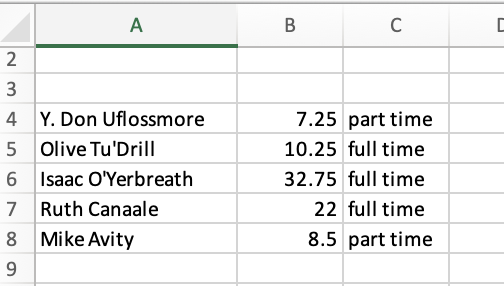
\includegraphics[keepaspectratio]{dentrpt1.png}}
\caption{Dental Report}
\end{figure}

Notice this is just exporting our data into an excel file without a shell, but we do place our data starting on line A4 and we do not export variable names.

We'll use the shell report called ``dentrpt1-skeleton.xlsx'', and we'll fill it out using Stata. This is just an example, but it can be easily applicable in many office settings. It is preferable to fill out the report this way, since if there is a mistake, then it is is easy to fix without generating a new report from scratch.
\pandocbounded{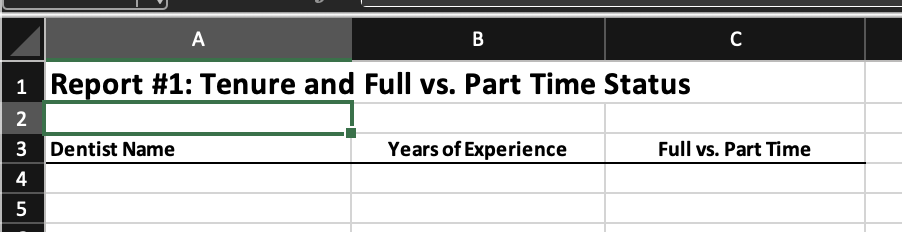
\includegraphics[keepaspectratio]{dentrpt2.png}}

First we'll use the copy command to copy the Report Shell over our newly created file called ``dentrpt1.xlsx''.

\begin{Shaded}
\begin{Highlighting}[]
\NormalTok{copy }\StringTok{"dentrpt1{-}skeleton.xlsx"} \StringTok{"dentrpt1.xlsx"}\NormalTok{, }\KeywordTok{replace}
\end{Highlighting}
\end{Shaded}

Now we will use the ``modify'' option to modify our report shell to fill out
the report with data.

\begin{Shaded}
\begin{Highlighting}[]
\KeywordTok{export}\NormalTok{ excel }\StringTok{"dentrpt1.xlsx"}\NormalTok{, sheet(}\StringTok{"dentists"}\NormalTok{, modify) cell(A4)}
\end{Highlighting}
\end{Shaded}

\begin{figure}
\centering
\pandocbounded{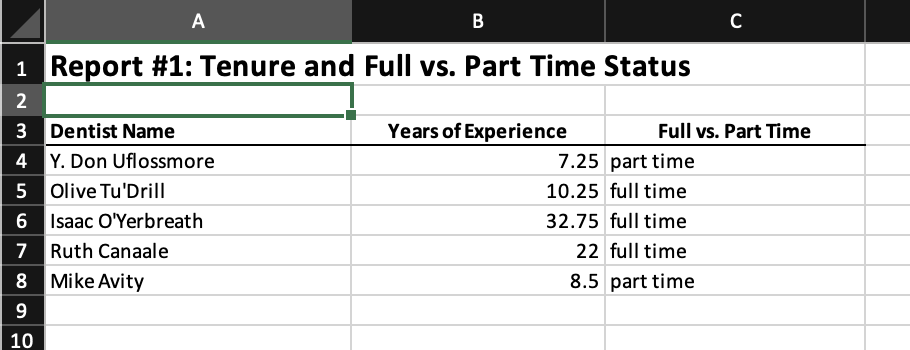
\includegraphics[keepaspectratio]{dentrpt3.png}}
\caption{Dental Report v3}
\end{figure}

Notice that there are two sheets in the report shell: ``dentists'' and ``Sheet2''. We modified the sheet called ``dentists'' and pasted our data in this sheet starting at cell A4.

We can format our formats, too. We have our report shell in ``dentrpt2-skeleton.xlsx''. We will do is similar to the first report, but we will add the keepcellfmt option.

\begin{Shaded}
\begin{Highlighting}[]
\NormalTok{copy }\StringTok{"dentrpt2{-}skeleton.xlsx"} \StringTok{"dentrpt2.xlsx"}\NormalTok{, }\KeywordTok{replace}
\KeywordTok{export}\NormalTok{ excel }\StringTok{"dentrpt2.xlsx"}\NormalTok{, sheet(}\StringTok{"dentists"}\NormalTok{, modify) cell(A4) keepcellfmt}
\end{Highlighting}
\end{Shaded}

Note: this keepcellfmt is unavailable in Stata 14, but you should have it in your newer version.

We'll do something similar, but we will include averages for years and full-time vs part time.

\begin{Shaded}
\begin{Highlighting}[]
\NormalTok{copy }\StringTok{"dentrpt3{-}skeleton.xlsx"} \StringTok{"dentrpt3.xlsx"}\NormalTok{, }\KeywordTok{replace}
\KeywordTok{export}\NormalTok{ excel }\StringTok{"dentrpt3.xlsx"}\NormalTok{, sheet(}\StringTok{"dentists"}\NormalTok{, modify) cell(A6) }
\end{Highlighting}
\end{Shaded}

\begin{figure}
\centering
\pandocbounded{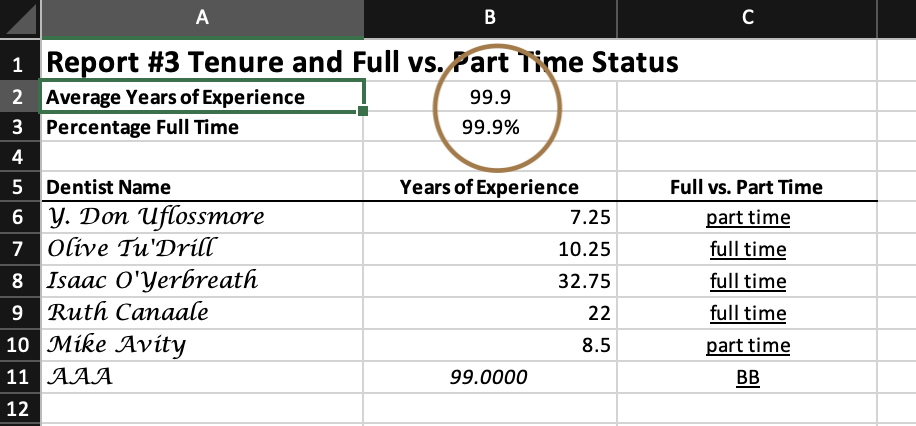
\includegraphics[keepaspectratio]{dentrpt5.png}}
\caption{Dental Report v5}
\end{figure}

You have two options for the percentages: 1) add average formula in Excel or 2) use put excel. It is easy to add formulas in excel, but what if the number of observation changes over time? Then, you would need to modify the Excel sheet. Using put excel you can update the averages without messing with formulas in excel.

It is poor practice to run the summarize command and manually entering it into your report. Use local macros and do it dynamically!

We will set our dentists report to be modified by Stata, and then run the summarize command and take the average stored after the command and put it into excel.

\begin{Shaded}
\begin{Highlighting}[]
\NormalTok{putexcel }\KeywordTok{set} \StringTok{"dentrpt3.xlsx"}\NormalTok{, sheet(}\StringTok{"dentists"}\NormalTok{) modify}
\end{Highlighting}
\end{Shaded}

After setting the sheet to be modified, we can write expression, returned results, formulas, graphs, scalars, matrices, etc.

Let's look at what the summarize command stores after being run.

\begin{Shaded}
\begin{Highlighting}[]
\KeywordTok{summarize}\NormalTok{ years}
\FunctionTok{return} \OtherTok{list}
\end{Highlighting}
\end{Shaded}

\begin{verbatim}
    Variable |        Obs        Mean    Std. Dev.       Min        Max
-------------+---------------------------------------------------------
       years |          5       16.15    10.98095       7.25      32.75


scalars:
                  r(N) =  5
              r(sum_w) =  5
               r(mean) =  16.15
                r(Var) =  120.58125
                 r(sd) =  10.98094941250528
                r(min) =  7.25
                r(max) =  32.75
                r(sum) =  80.75
\end{verbatim}

There are several scalars that are stored, such as number of observations r(N), mean r(mean), standard deviation r(sd), etc.
If we use the detail option, we'll see more scalars.

We can retreive those scalars with local macros, such as `r(mean)'.

\begin{Shaded}
\begin{Highlighting}[]
\NormalTok{summarize years}
\NormalTok{putexcel B2 = \textasciigrave{}r(mean)\textquotesingle{}}
\NormalTok{summarize fulltime}
\NormalTok{putexcel B3 = \textasciigrave{}r(mean)\textquotesingle{}}
\NormalTok{putexcel save //Not in older version}
\end{Highlighting}
\end{Shaded}

\begin{figure}
\centering
\pandocbounded{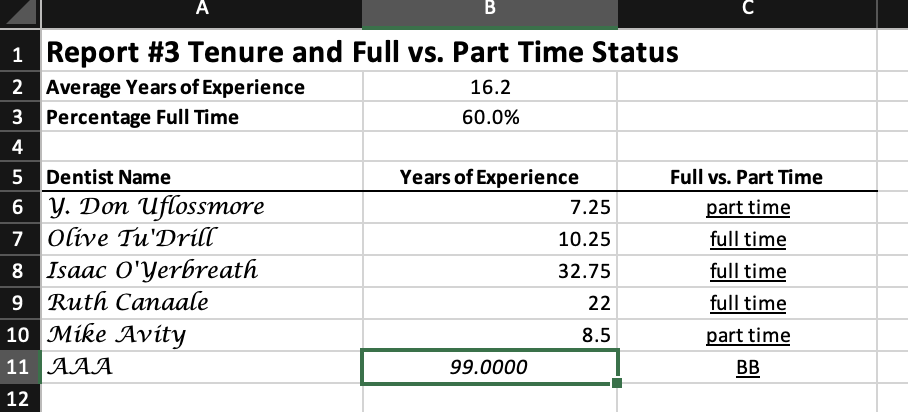
\includegraphics[keepaspectratio]{dentrpt6.png}}
\caption{Dental Report v6}
\end{figure}

More on Putexcel
\url{https://blog.stata.com/2017/01/10/creating-excel-tables-with-putexcel-part-1-introduction-and-formatting/}

\chapter{Cleaning and Checking Data}\label{cleaning-and-checking-data}

\emph{Mitchell Chapter 4}

Good note from Mitchell at the beginning: Garbage In; Garbage Out.

Before doing analysis, you really need to check your data to look for data quality issues.

\section{Checking individual variables}\label{checking-individual-variables}

We start off with looking from problems in individual variables. Mitchell uses Working Women's Survey (WWS) dataset, but we'll use Current Population Survey (CPS) data, as well.

\begin{Shaded}
\begin{Highlighting}[]
\KeywordTok{use}\NormalTok{ wws, }\KeywordTok{clear}
\end{Highlighting}
\end{Shaded}

The \emph{describe} command is a useful command to see an overview of your data
with variables labels, storage type, and value lables (if any)

\begin{Shaded}
\begin{Highlighting}[]
\KeywordTok{quietly}\NormalTok{ cd }\StringTok{"/Users/Sam/Desktop/Data/CPS/"}
\KeywordTok{use}\NormalTok{ smalljul25pub}
\KeywordTok{describe}
\end{Highlighting}
\end{Shaded}

\begin{verbatim}
Contains data from smalljul25pub.dta
  obs:       122,252                          
 vars:            50                          12 Aug 2025 19:17
 size:     8,313,136                          
------------------------------------------------------------------------------------------------------------------
              storage   display    value
variable name   type    format     label      variable label
------------------------------------------------------------------------------------------------------------------
hrhhid2         int     %8.0g                 
hrmis           byte    %8.0g                 HRMIS
hrmonth         byte    %8.0g                 HRMONTH
hryear4         int     %8.0g                 HRYEAR4
gestfips        byte    %8.0g                 
gediv           byte    %8.0g                 
pulineno        byte    %8.0g                 PULINENO
pudis           byte    %8.0g                 PUDIS
puiodp1         byte    %8.0g                 PUIODP1
puiodp2         byte    %8.0g                 PUIODP2
puiodp3         byte    %8.0g                 PUIODP3
perrp           byte    %8.0g                 
pesex           byte    %8.0g                 
pemaritl        byte    %8.0g                 
pehspnon        byte    %8.0g                 
peeduca         byte    %8.0g                 
peafever        byte    %8.0g                 
ptdtrace        byte    %8.0g                 
prpertyp        byte    %8.0g                 
prtage          byte    %8.0g                 
pehractt        int     %8.0g                 
pehract1        byte    %8.0g                 
pehract2        byte    %8.0g                 
pemlr           byte    %8.0g                 
peio1icd        int     %8.0g                 
peio1cow        byte    %8.0g                 
peio2cow        byte    %8.0g                 
prmjind1        byte    %8.0g                 
prmjind2        byte    %8.0g                 
prmjocc1        byte    %8.0g                 
prmjocc2        byte    %8.0g                 
prdtind1        byte    %8.0g                 
prdtind2        byte    %8.0g                 
prdtocc1        byte    %8.0g                 
prdtocc2        byte    %8.0g                 
prsjmj          byte    %8.0g                 
peernhry        byte    %8.0g                 
peernhro        byte    %8.0g                 
peernlab        byte    %8.0g                 
prerelg         byte    %8.0g                 
prdisflg        byte    %8.0g                 
pecert1         byte    %8.0g                 
pecert2         byte    %8.0g                 
pecert3         byte    %8.0g                 
pwcmpwgt        long    %12.0g                
pternwa         long    %12.0g                
ptio1ocd        int     %8.0g                 
hrhhid          double  %10.0g                
ptwk            byte    %8.0g                 
gtmetsta        byte    %8.0g                 
------------------------------------------------------------------------------------------------------------------
Sorted by: 
\end{verbatim}

You will noticed that we lack value labels and variable labels. Luckily we have a data dictionary on Census's website. Let's label the variables and use the \emph{describe} command again.

\begin{Shaded}
\begin{Highlighting}[]
\KeywordTok{label} \KeywordTok{variable}\NormalTok{ gestfips }\StringTok{"State"}
\KeywordTok{label} \KeywordTok{variable}\NormalTok{ gediv }\StringTok{"Census Region"}
\KeywordTok{label} \KeywordTok{variable}\NormalTok{ pternwa }\StringTok{"Weekly earnings"}
\KeywordTok{label} \KeywordTok{variable}\NormalTok{ peio1cow }\StringTok{"Class of worker in Main Job"}
\KeywordTok{label} \KeywordTok{variable}\NormalTok{ peio1cow }\StringTok{"Class of worker in Second Job"}
\KeywordTok{label} \KeywordTok{variable}\NormalTok{ pemlr }\StringTok{"Labor Force Status"}
\KeywordTok{describe}
\end{Highlighting}
\end{Shaded}

\begin{verbatim}
Contains data from smalljul25pub.dta
  obs:       122,252                          
 vars:            50                          12 Aug 2025 19:17
 size:     8,313,136                          
------------------------------------------------------------------------------------------------------------------
              storage   display    value
variable name   type    format     label      variable label
------------------------------------------------------------------------------------------------------------------
hrhhid2         int     %8.0g                 
hrmis           byte    %8.0g                 HRMIS
hrmonth         byte    %8.0g                 HRMONTH
hryear4         int     %8.0g                 HRYEAR4
gestfips        byte    %8.0g                 State
gediv           byte    %8.0g                 Census Region
pulineno        byte    %8.0g                 PULINENO
pudis           byte    %8.0g                 PUDIS
puiodp1         byte    %8.0g                 PUIODP1
puiodp2         byte    %8.0g                 PUIODP2
puiodp3         byte    %8.0g                 PUIODP3
perrp           byte    %8.0g                 
pesex           byte    %8.0g                 
pemaritl        byte    %8.0g                 
pehspnon        byte    %8.0g                 
peeduca         byte    %8.0g                 
peafever        byte    %8.0g                 
ptdtrace        byte    %8.0g                 
prpertyp        byte    %8.0g                 
prtage          byte    %8.0g                 
pehractt        int     %8.0g                 
pehract1        byte    %8.0g                 
pehract2        byte    %8.0g                 
pemlr           byte    %8.0g                 Labor Force Status
peio1icd        int     %8.0g                 
peio1cow        byte    %8.0g                 Class of worker in Second Job
peio2cow        byte    %8.0g                 
prmjind1        byte    %8.0g                 
prmjind2        byte    %8.0g                 
prmjocc1        byte    %8.0g                 
prmjocc2        byte    %8.0g                 
prdtind1        byte    %8.0g                 
prdtind2        byte    %8.0g                 
prdtocc1        byte    %8.0g                 
prdtocc2        byte    %8.0g                 
prsjmj          byte    %8.0g                 
peernhry        byte    %8.0g                 
peernhro        byte    %8.0g                 
peernlab        byte    %8.0g                 
prerelg         byte    %8.0g                 
prdisflg        byte    %8.0g                 
pecert1         byte    %8.0g                 
pecert2         byte    %8.0g                 
pecert3         byte    %8.0g                 
pwcmpwgt        long    %12.0g                
pternwa         long    %12.0g                Weekly earnings
ptio1ocd        int     %8.0g                 
hrhhid          double  %10.0g                
ptwk            byte    %8.0g                 
gtmetsta        byte    %8.0g                 
------------------------------------------------------------------------------------------------------------------
Sorted by: 
\end{verbatim}

\section{One way tabulation}\label{one-way-tabulation}

The \emph{tabulation} or \emph{tab} command is very useful to inspect categorical variables.

The tabulation or tab command is very useful to inspect categorical variables.
Let's look at collgrad, which is a binary for college graduate status in wws data, and let's look at race data, which is a categorical variable. Let's include the missing option to make sure no observations are missing data

\begin{Shaded}
\begin{Highlighting}[]
\KeywordTok{quietly}\NormalTok{ cd }\StringTok{"/Users/Sam/Desktop/Econ 645/Data/Mitchell"}
\KeywordTok{use}\NormalTok{ wws, }\KeywordTok{clear}
\KeywordTok{tabulate}\NormalTok{ collgrad, }\FunctionTok{missing}
\KeywordTok{tabulate}\NormalTok{ race, }\FunctionTok{missing}
\end{Highlighting}
\end{Shaded}

\begin{verbatim}
(Working Women Survey)

    college |
   graduate |      Freq.     Percent        Cum.
------------+-----------------------------------
          0 |      1,713       76.27       76.27
          1 |        533       23.73      100.00
------------+-----------------------------------
      Total |      2,246      100.00

       race |      Freq.     Percent        Cum.
------------+-----------------------------------
          1 |      1,636       72.84       72.84
          2 |        583       25.96       98.80
          3 |         26        1.16       99.96
          4 |          1        0.04      100.00
------------+-----------------------------------
      Total |      2,246      100.00
\end{verbatim}

Race should only be coded between 1 and 3, so we have one miscoded observation.
Let's find the observation's idcode

\begin{Shaded}
\begin{Highlighting}[]
\OtherTok{list}\NormalTok{ idcode race }\KeywordTok{if}\NormalTok{ race==4}
\end{Highlighting}
\end{Shaded}

\begin{verbatim}
(Working Women Survey)

      +---------------+
      | idcode   race |
      |---------------|
2013. |    543      4 |
      +---------------+
\end{verbatim}

\section{Summarize}\label{summarize}

The \emph{summarize} or \emph{sum} command is very useful to inspect continuous variables. Let's look at the amount of unemployment insurance in unempins. The values range between 0 and 300 dollars for unemployed insurance received last week.

\begin{Shaded}
\begin{Highlighting}[]
\KeywordTok{quietly}\NormalTok{ cd }\StringTok{"/Users/Sam/Desktop/Econ 645/Data/Mitchell"}
\KeywordTok{use}\NormalTok{ wws, }\KeywordTok{clear}
\KeywordTok{summarize}\NormalTok{ unempins}
\end{Highlighting}
\end{Shaded}

\begin{verbatim}
(Working Women Survey)

    Variable |        Obs        Mean    Std. Dev.       Min        Max
-------------+---------------------------------------------------------
    unempins |      2,246    30.50401    73.16682          0        299
\end{verbatim}

Let's look at weekly earnings in CPS.

\begin{Shaded}
\begin{Highlighting}[]
\KeywordTok{quietly}\NormalTok{ cd }\StringTok{"/Users/Sam/Desktop/Data/CPS/"}
\KeywordTok{use}\NormalTok{ smalljul25pub.dta, }\KeywordTok{replace}
\KeywordTok{gen}\NormalTok{ earnings=pternwa/100}
\KeywordTok{summarize}\NormalTok{ earnings }\KeywordTok{if}\NormalTok{ prerelg==1}
\end{Highlighting}
\end{Shaded}

\begin{verbatim}
(28,617 missing values generated)

    Variable |        Obs        Mean    Std. Dev.       Min        Max
-------------+---------------------------------------------------------
    earnings |      9,635    1408.951     1251.25          0    6930.64
\end{verbatim}

The data range between \$0 and \$6,930.64 in weekly earnings last week with a mean of 1,408.95 dollars and a standard deviation of 1,251,25 dollars. The max seems
a bit high. Let's add the detail option to get more information.

\begin{Shaded}
\begin{Highlighting}[]
\KeywordTok{summarize}\NormalTok{ earnings }\KeywordTok{if}\NormalTok{ prerelg==1, }\KeywordTok{detail}
\end{Highlighting}
\end{Shaded}

\begin{verbatim}
                          earnings
-------------------------------------------------------------
      Percentiles      Smallest
 1%           88              0
 5%          250              0
10%          384              0       Obs               9,635
25%          680              0       Sum of Wgt.       9,635

50%         1060                      Mean           1408.951
                        Largest       Std. Dev.       1251.25
75%         1730        6930.64
90%         2700        6930.64       Variance        1565626
95%         3460        6930.64       Skewness       2.688217
99%      6930.64        6930.64       Kurtosis        11.9109
\end{verbatim}

We can see that the mean is \$1,408.95, while the median is \$1,060.00. The mean appears to be skewed rightward, where the skewness is 2.7 and the kurtosis is 11.9. The 95th percentile is 3,460.00 while the 99th percentile is \$6,930.64.

Let's look at wage data in the wws data set

\begin{Shaded}
\begin{Highlighting}[]
\KeywordTok{quietly}\NormalTok{ cd }\StringTok{"/Users/Sam/Desktop/Econ 645/Data/Mitchell"}
\KeywordTok{use}\NormalTok{ wws, }\KeywordTok{clear}
\KeywordTok{summarize}\NormalTok{ wage, }\KeywordTok{detail}
\end{Highlighting}
\end{Shaded}

\begin{verbatim}
(Working Women Survey)

                         hourly wage
-------------------------------------------------------------
      Percentiles      Smallest
 1%     1.892108              0
 5%     2.801002       1.004952
10%     3.220612       1.032247       Obs               2,246
25%     4.259257       1.151368       Sum of Wgt.       2,246

50%     6.276297                      Mean           288.2885
                        Largest       Std. Dev.      9595.692
75%     9.661837       40.19808
90%     12.77777       40.74659       Variance       9.21e+07
95%     16.73912         250000       Skewness       35.45839
99%     38.70926         380000       Kurtosis       1297.042
\end{verbatim}

For our wws data, our mean of 288.29 dollars/hour appears to be highly skewed rightward and heavily influenced by outliers. Our median hourly wage is 6.7 dollars per hour and our 99th percentile hourly wage is 38.7 dollars per hour, but our mean is 288.29 dollar/hour. Our skewness is 35, which means our wage data are highly skewed. Our Kurtosis shows that the max outliers are heavily skewing the results. A normal distributed variable should have a kurtosis of 3, and our kurtosis is 1297. When we see the 2 largets observations, they are 250,000 and 380,000 dollars/hour.

This means we have found potential data measurement issues. Let's look at the outliers

\begin{Shaded}
\begin{Highlighting}[]
\KeywordTok{quietly}\NormalTok{ cd }\StringTok{"/Users/Sam/Desktop/Econ 645/Data/Mitchell"}
\KeywordTok{quietly} \KeywordTok{use}\NormalTok{ wws, }\KeywordTok{clear}
\OtherTok{list}\NormalTok{ idcode wage }\KeywordTok{if}\NormalTok{ wage \textgreater{} 1000}
\end{Highlighting}
\end{Shaded}

\begin{verbatim}
      | idcode     wage |
      |-----------------|
 893. |   3145   380000 |
1241. |   2341   250000 |
      +-----------------+
\end{verbatim}

Let's look at ages, which should range frm 21 to 50 years old. We can use both
the \emph{summarize} and \emph{tabulate} commands. \emph{Tabulate} can be very useful with
continuous variables if the range is not too large.

\begin{Shaded}
\begin{Highlighting}[]
\KeywordTok{quietly}\NormalTok{ cd }\StringTok{"/Users/Sam/Desktop/Econ 645/Data/Mitchell"}
\KeywordTok{quietly} \KeywordTok{use}\NormalTok{ wws, }\KeywordTok{clear}
\KeywordTok{summarize}\NormalTok{ age}
\KeywordTok{tabulate}\NormalTok{ age}
\end{Highlighting}
\end{Shaded}

\begin{verbatim}
    Variable |        Obs        Mean    Std. Dev.       Min        Max
-------------+---------------------------------------------------------
         age |      2,246    36.25111    5.437983         21         83

     age in |
    current |
       year |      Freq.     Percent        Cum.
------------+-----------------------------------
         21 |          2        0.09        0.09
         22 |          8        0.36        0.45
         23 |         16        0.71        1.16
         24 |         35        1.56        2.72
         25 |         44        1.96        4.67
         26 |         50        2.23        6.90
         27 |         50        2.23        9.13
         28 |         63        2.80       11.93
         29 |         49        2.18       14.11
         30 |         55        2.45       16.56
         31 |         57        2.54       19.10
         32 |         60        2.67       21.77
         33 |         56        2.49       24.27
         34 |         95        4.23       28.50
         35 |        213        9.48       37.98
         36 |        224        9.97       47.95
         37 |        171        7.61       55.57
         38 |        175        7.79       63.36
         39 |        167        7.44       70.79
         40 |        139        6.19       76.98
         41 |        148        6.59       83.57
         42 |        111        4.94       88.51
         43 |        110        4.90       93.41
         44 |         98        4.36       97.77
         45 |         45        2.00       99.78
         46 |          1        0.04       99.82
         47 |          1        0.04       99.87
         48 |          1        0.04       99.91
         54 |          1        0.04       99.96
         83 |          1        0.04      100.00
------------+-----------------------------------
      Total |      2,246      100.00
\end{verbatim}

Let's look at the outliers

\begin{Shaded}
\begin{Highlighting}[]
\KeywordTok{quietly}\NormalTok{ cd }\StringTok{"/Users/Sam/Desktop/Econ 645/Data/Mitchell"}
\KeywordTok{quietly} \KeywordTok{use}\NormalTok{ wws, }\KeywordTok{clear}
\OtherTok{list}\NormalTok{ idcode age }\KeywordTok{if}\NormalTok{ age \textgreater{} 50}
\end{Highlighting}
\end{Shaded}

\begin{verbatim}
      | idcode   age |
      |--------------|
2205. |     80    54 |
2219. |     51    83 |
      +--------------+
\end{verbatim}

We have again found potential data measurement problems. The data is supposed to range from 21 to 50, but there are two observations with 54 and 83. It is possible that they were incorrectly entered, and they are supposed to be 45 and 38, respectively.

\section{Crosstabulation - categorical by categorical variables}\label{crosstabulation---categorical-by-categorical-variables}

The two-way tabulation through the \emph{tabulate} command is a very useful way to look for data quality problems or to double check binaries created. Let's look at variables metro, which is a binary for whether or not the observation lives in a metropolitian areas, and ccity, which is whether or not the observation lives in the center of the city.

\begin{Shaded}
\begin{Highlighting}[]
\KeywordTok{quietly}\NormalTok{ cd }\StringTok{"/Users/Sam/Desktop/Econ 645/Data/Mitchell"}
\KeywordTok{quietly} \KeywordTok{use}\NormalTok{ wws, }\KeywordTok{clear}
\KeywordTok{tabulate}\NormalTok{ metro ccity, }\FunctionTok{missing}
\end{Highlighting}
\end{Shaded}

\begin{verbatim}
Does woman |
   live in |  Does woman live in
     metro |     city center?
     area? |         0          1 |     Total
-----------+----------------------+----------
         0 |       665          0 |       665 
         1 |       926        655 |     1,581 
-----------+----------------------+----------
     Total |     1,591        655 |     2,246 
\end{verbatim}

An alternative is to count the number of observations that shouldn't be there. So we'll count the number of observations not in a metro area but in a city center. I personally don't use it, but it has it's uses.

\begin{Shaded}
\begin{Highlighting}[]
\KeywordTok{quietly}\NormalTok{ cd }\StringTok{"/Users/Sam/Desktop/Econ 645/Data/Mitchell"}
\KeywordTok{quietly} \KeywordTok{use}\NormalTok{ wws, }\KeywordTok{clear}
\FunctionTok{count} \KeywordTok{if}\NormalTok{ metro==0 \& ccity==1}
\end{Highlighting}
\end{Shaded}

\begin{verbatim}
  0
\end{verbatim}

Let's look at married and nevermarriaged. There should be no individuals that appear in both married and nevermarried.

\begin{Shaded}
\begin{Highlighting}[]
\KeywordTok{quietly}\NormalTok{ cd }\StringTok{"/Users/Sam/Desktop/Econ 645/Data/Mitchell"}
\KeywordTok{quietly} \KeywordTok{use}\NormalTok{ wws, }\KeywordTok{clear}
\KeywordTok{tabulate}\NormalTok{ married nevermarried, }\FunctionTok{missing}
\end{Highlighting}
\end{Shaded}

\begin{verbatim}
           |   Woman never been
           |        married
   married |         0          1 |     Total
-----------+----------------------+----------
         0 |       570        234 |       804 
         1 |     1,440          2 |     1,442 
-----------+----------------------+----------
     Total |     2,010        236 |     2,246 
\end{verbatim}

There may be observation that have been married, but not currently married. There should be no observations that are both married and never married.

\begin{Shaded}
\begin{Highlighting}[]
\KeywordTok{quietly}\NormalTok{ cd }\StringTok{"/Users/Sam/Desktop/Econ 645/Data/Mitchell"}
\KeywordTok{quietly} \KeywordTok{use}\NormalTok{ wws, }\KeywordTok{clear}
\FunctionTok{count} \KeywordTok{if}\NormalTok{ married == 1 \& nevermarried == 1}
\OtherTok{list}\NormalTok{ idcode married nevermarried }\KeywordTok{if}\NormalTok{ married == 1 \& nevermarried == 1}
\end{Highlighting}
\end{Shaded}

\begin{verbatim}
  2

      +-----------------------------+
      | idcode   married   neverm~d |
      |-----------------------------|
1523. |   1758         1          1 |
2231. |     22         1          1 |
      +-----------------------------+
\end{verbatim}

We have found another potential data measurement issue. There are 2 observations that are married and never married.

Let's look at college graduates and years of school completed. We can use \emph{tabulate} or the \emph{table} commands. I personally prefer \emph{tabulate}, since we can look for missing.

\begin{Shaded}
\begin{Highlighting}[]
\KeywordTok{quietly}\NormalTok{ cd }\StringTok{"/Users/Sam/Desktop/Econ 645/Data/Mitchell"}
\KeywordTok{quietly} \KeywordTok{use}\NormalTok{ wws, }\KeywordTok{clear}
\KeywordTok{tabulate}\NormalTok{ yrschool collgrad, }\FunctionTok{missing}
\end{Highlighting}
\end{Shaded}

\begin{verbatim}
  Years of |
    school |   college graduate
 completed |         0          1 |     Total
-----------+----------------------+----------
         8 |        69          1 |        70 
         9 |        55          0 |        55 
        10 |        84          0 |        84 
        11 |       123          0 |       123 
        12 |       943          0 |       943 
        13 |       174          2 |       176 
        14 |       180          7 |       187 
        15 |        81         11 |        92 
        16 |         0        252 |       252 
        17 |         0        106 |       106 
        18 |         0        154 |       154 
         . |         4          0 |         4 
-----------+----------------------+----------
     Total |     1,713        533 |     2,246 
\end{verbatim}

We can use the \emph{table} command

\begin{Shaded}
\begin{Highlighting}[]
\KeywordTok{table}\NormalTok{ yrschool collgrad}
\end{Highlighting}
\end{Shaded}

\begin{verbatim}
Years of  |  college  
school    |  graduate 
completed |    0     1
----------+-----------
        8 |   69     1
        9 |   55      
       10 |   84      
       11 |  123      
       12 |  943      
       13 |  174     2
       14 |  180     7
       15 |   81    11
       16 |        252
       17 |        106
       18 |        154
----------------------
\end{verbatim}

Now let's find the ID with potential problems

\begin{Shaded}
\begin{Highlighting}[]
\OtherTok{list}\NormalTok{ idcode }\KeywordTok{if}\NormalTok{ yrschool \textless{} 16 \& collgrad == 1}
\end{Highlighting}
\end{Shaded}

\begin{verbatim}
      | idcode |
      |--------|
 195. |   4721 |
 369. |   4334 |
 464. |   4131 |
 553. |   3929 |
 690. |   3589 |
      |--------|
1092. |   2681 |
1098. |   2674 |
1114. |   2640 |
1124. |   2613 |
1221. |   2384 |
      |--------|
1493. |   1810 |
1829. |    993 |
1843. |    972 |
1972. |    689 |
2114. |    312 |
      |--------|
2174. |    172 |
2198. |    107 |
2215. |     63 |
2228. |     25 |
2229. |     24 |
      |--------|
2230. |     23 |
      +--------+
\end{verbatim}

There is at least one potential measurement problem. There is an observation with 8 years of schooling completed listed as a college graduate. We also see that there are 2 observations with 13 years and 7 with 14 years. These may be two-year college graduates, and these observations may not be problematic.

\section{Checking categorical by continuous variables}\label{checking-categorical-by-continuous-variables}

It is also helpful to look at continuous variables by different categories. Let's look at the binary variable for union, if the observation is a union member or not by uniondues.

\begin{Shaded}
\begin{Highlighting}[]
\KeywordTok{quietly}\NormalTok{ cd }\StringTok{"/Users/Sam/Desktop/Econ 645/Data/Mitchell"}
\KeywordTok{quietly} \KeywordTok{use}\NormalTok{ wws, }\KeywordTok{clear}
\KeywordTok{summarize}\NormalTok{ uniondues, }\KeywordTok{detail}
\end{Highlighting}
\end{Shaded}

\begin{verbatim}
                  Union Dues paid last week
-------------------------------------------------------------
      Percentiles      Smallest
 1%            0              0
 5%            0              0
10%            0              0       Obs               2,242
25%            0              0       Sum of Wgt.       2,242

50%            0                      Mean           5.603479
                        Largest       Std. Dev.      9.029045
75%           10             29
90%           22             29       Variance       81.52365
95%           26             29       Skewness        1.35268
99%           29             29       Kurtosis       3.339635
\end{verbatim}

The median union dues is 0 dollars, which makes sense. The meand is 5.6 dollars, while the maximum value is 29 dollars.

Let's use the \emph{bysort} command, which will sort our data by the categorical variable specified.

\begin{Shaded}
\begin{Highlighting}[]
\KeywordTok{quietly}\NormalTok{ cd }\StringTok{"/Users/Sam/Desktop/Econ 645/Data/Mitchell"}
\KeywordTok{quietly} \KeywordTok{use}\NormalTok{ wws, }\KeywordTok{clear}
\KeywordTok{bysort} \KeywordTok{union}\NormalTok{: }\KeywordTok{summarize}\NormalTok{ uniondues}
\end{Highlighting}
\end{Shaded}

\begin{verbatim}
-> union = 0

    Variable |        Obs        Mean    Std. Dev.       Min        Max
-------------+---------------------------------------------------------
   uniondues |      1,413     .094126    1.502237          0         27

------------------------------------------------------------------------------------------------------------------
-> union = 1

    Variable |        Obs        Mean    Std. Dev.       Min        Max
-------------+---------------------------------------------------------
   uniondues |        461    14.65944    8.707759          0         29

------------------------------------------------------------------------------------------------------------------
-> union = .

    Variable |        Obs        Mean    Std. Dev.       Min        Max
-------------+---------------------------------------------------------
   uniondues |        368    15.41304    8.815582          0         29
\end{verbatim}

The mean for not in a union is less than 1 dollar with 1,413 observations
The mean for union is about 15 dollars with 461 observations
The mean for missing is about 15 dollars with 368 observations

\begin{Shaded}
\begin{Highlighting}[]
\KeywordTok{quietly}\NormalTok{ cd }\StringTok{"/Users/Sam/Desktop/Econ 645/Data/Mitchell"}
\KeywordTok{quietly} \KeywordTok{use}\NormalTok{ wws, }\KeywordTok{clear}
\KeywordTok{tabulate}\NormalTok{ uniondues }\KeywordTok{if} \KeywordTok{union}\NormalTok{==0, }\FunctionTok{missing}
\end{Highlighting}
\end{Shaded}

\begin{verbatim}
 Union Dues |
  paid last |
       week |      Freq.     Percent        Cum.
------------+-----------------------------------
          0 |      1,407       99.29       99.29
         10 |          1        0.07       99.36
         17 |          1        0.07       99.44
         26 |          2        0.14       99.58
         27 |          2        0.14       99.72
          . |          4        0.28      100.00
------------+-----------------------------------
      Total |      1,417      100.00
\end{verbatim}

We see about 4 observations have union dues. We may or may not need to recode them to 0. It is possible that someone may be not be a union members, but still have to pay an agency fee. Let's assume that they are not in 14(b) state..

The recode command can to create a new variable if a person pay union dues. Now let's compare union members to those who pay union dues

\begin{Shaded}
\begin{Highlighting}[]
\KeywordTok{quietly}\NormalTok{ cd }\StringTok{"/Users/Sam/Desktop/Econ 645/Data/Mitchell"}
\KeywordTok{quietly} \KeywordTok{use}\NormalTok{ wws, }\KeywordTok{clear}
\KeywordTok{recode}\NormalTok{ uniondues (0=0) (1/}\FunctionTok{max}\NormalTok{=1), }\KeywordTok{generate}\NormalTok{(paysdues)}
\KeywordTok{tabulate} \KeywordTok{union}\NormalTok{ paysdues, }\FunctionTok{missing}
\end{Highlighting}
\end{Shaded}

\begin{verbatim}
(784 differences between uniondues and paysdues)

           | RECODE of uniondues (Union Dues
     union |         paid last week)
    worker |         0          1          . |     Total
-----------+---------------------------------+----------
         0 |     1,407          6          4 |     1,417 
         1 |        17        444          0 |       461 
         . |         7        361          0 |       368 
-----------+---------------------------------+----------
     Total |     1,431        811          4 |     2,246 
\end{verbatim}

Let's list the non-union members paying union dues.
Note: we use the abb(\#) option to abbreviate the observation to 20 characters

\begin{Shaded}
\begin{Highlighting}[]
\OtherTok{list}\NormalTok{ idcode }\KeywordTok{union}\NormalTok{ uniondues }\KeywordTok{if} \KeywordTok{union}\NormalTok{==0 \& (uniondues \textgreater{} 0) \& !}\FunctionTok{missing}\NormalTok{(uniondues), abb(20)}
\end{Highlighting}
\end{Shaded}

\begin{verbatim}
      | idcode   union   uniondues |
      |----------------------------|
 561. |   3905       0          10 |
 582. |   3848       0          26 |
 736. |   3464       0          17 |
1158. |   2541       0          27 |
1668. |   1411       0          27 |
      |----------------------------|
2100. |    345       0          26 |
      +----------------------------+
\end{verbatim}

Let's look at another great command for observing categorical and continuous
variables together: \emph{tabstat}

We could use \emph{tab} with a sum option

\begin{Shaded}
\begin{Highlighting}[]
\KeywordTok{quietly}\NormalTok{ cd }\StringTok{"/Users/Sam/Desktop/Econ 645/Data/Mitchell"}
\KeywordTok{quietly} \KeywordTok{use}\NormalTok{ wws, }\KeywordTok{clear}
\KeywordTok{tab}\NormalTok{ married, }\KeywordTok{sum}\NormalTok{(marriedyrs)}
\end{Highlighting}
\end{Shaded}

\begin{verbatim}
            |  Summary of Years married (rounded
            |          to nearest year)
    married |        Mean   Std. Dev.       Freq.
------------+------------------------------------
          0 |           0           0         804
          1 |   5.5409154   3.5521383       1,442
------------+------------------------------------
      Total |   3.5574354   3.8933494       2,246
\end{verbatim}

Or, we can use \emph{tabstat} which gives us more options

\begin{Shaded}
\begin{Highlighting}[]
\KeywordTok{quietly}\NormalTok{ cd }\StringTok{"/Users/Sam/Desktop/Econ 645/Data/Mitchell"}
\KeywordTok{quietly} \KeywordTok{use}\NormalTok{ wws, }\KeywordTok{clear}
\KeywordTok{tabstat}\NormalTok{ marriedyrs, }\KeywordTok{by}\NormalTok{(married) }\KeywordTok{statistics}\NormalTok{(n }\KeywordTok{mean} \FunctionTok{sd} \FunctionTok{min} \FunctionTok{max}\NormalTok{ p25 p50 p75) }\FunctionTok{missing}
\end{Highlighting}
\end{Shaded}

\begin{verbatim}
Summary for variables: marriedyrs
     by categories of: married (married)

 married |         N      mean        sd       min       max       p25       p50       p75
---------+--------------------------------------------------------------------------------
       0 |       804         0         0         0         0         0         0         0
       1 |      1442  5.540915  3.552138         0        11         2         6         9
---------+--------------------------------------------------------------------------------
   Total |      2246  3.557435  3.893349         0        11         0         2         7
------------------------------------------------------------------------------------------
\end{verbatim}

No observation that said they were never married reported years of marriage

Let's look at current years of experience and everworked binary

\begin{Shaded}
\begin{Highlighting}[]
\KeywordTok{quietly}\NormalTok{ cd }\StringTok{"/Users/Sam/Desktop/Econ 645/Data/Mitchell"}
\KeywordTok{quietly} \KeywordTok{use}\NormalTok{ wws, }\KeywordTok{clear}
\KeywordTok{tabstat}\NormalTok{ currexp, }\KeywordTok{by}\NormalTok{(everworked) }\KeywordTok{statistics}\NormalTok{(n }\KeywordTok{mean} \FunctionTok{sd} \FunctionTok{min} \FunctionTok{max}\NormalTok{) }\FunctionTok{missing}
\end{Highlighting}
\end{Shaded}

\begin{verbatim}
Summary for variables: currexp
     by categories of: everworked (Has woman ever worked?)

everworked |         N      mean        sd       min       max
-----------+--------------------------------------------------
         0 |        60         0         0         0         0
         1 |      2171  5.328881  5.042181         0        26
-----------+--------------------------------------------------
     Total |      2231  5.185567  5.048073         0        26
--------------------------------------------------------------
\end{verbatim}

Let's total years of experience, which is currexp plus prevexp

\begin{Shaded}
\begin{Highlighting}[]
\KeywordTok{quietly}\NormalTok{ cd }\StringTok{"/Users/Sam/Desktop/Econ 645/Data/Mitchell"}
\KeywordTok{quietly} \KeywordTok{use}\NormalTok{ wws, }\KeywordTok{clear}
\KeywordTok{generate}\NormalTok{ totexp=currexp+prevexp}
\KeywordTok{tabstat}\NormalTok{ totexp, }\KeywordTok{by}\NormalTok{(everworked) }\KeywordTok{statistics}\NormalTok{(n }\KeywordTok{mean} \FunctionTok{sd} \FunctionTok{min} \FunctionTok{max}\NormalTok{) }\FunctionTok{missing}
\end{Highlighting}
\end{Shaded}

\begin{verbatim}
(15 missing values generated)


Summary for variables: totexp
     by categories of: everworked (Has woman ever worked?)

everworked |         N      mean        sd       min       max
-----------+--------------------------------------------------
         0 |        60         0         0         0         0
         1 |      2171  11.57761  4.552392         1        29
-----------+--------------------------------------------------
     Total |      2231  11.26625  4.865816         0        29
--------------------------------------------------------------
\end{verbatim}

Everyone with at least one year experience has experience working

\textbf{Note:}
Three ways to
1. bysort x\_cat: summarize x\_con
2. tab x\_cat, sum(x\_con)
3. tabstat x\_con, by(x\_cat) statistics(\ldots)

\section{Checking continuous by continuous variables}\label{checking-continuous-by-continuous-variables}

We will compare two continuous variables to continuous variables Let's look at unemployment insuranced received last week if the hours were greater than 30 and hours are not missing.

\begin{Shaded}
\begin{Highlighting}[]
\KeywordTok{quietly}\NormalTok{ cd }\StringTok{"/Users/Sam/Desktop/Econ 645/Data/Mitchell"}
\KeywordTok{quietly} \KeywordTok{use}\NormalTok{ wws, }\KeywordTok{clear}
\KeywordTok{summarize}\NormalTok{ unempins }\KeywordTok{if}\NormalTok{ hours \textgreater{} 30 \& !}\FunctionTok{missing}\NormalTok{(hours)}
\end{Highlighting}
\end{Shaded}

\begin{verbatim}
    Variable |        Obs        Mean    Std. Dev.       Min        Max
-------------+---------------------------------------------------------
    unempins |      1,800    1.333333    16.04617          0        287
\end{verbatim}

The mean is around 1.3 and our range is between our expected 0 and 287

\begin{Shaded}
\begin{Highlighting}[]
\KeywordTok{quietly}\NormalTok{ cd }\StringTok{"/Users/Sam/Desktop/Econ 645/Data/Mitchell"}
\KeywordTok{quietly} \KeywordTok{use}\NormalTok{ wws, }\KeywordTok{clear}
\FunctionTok{count} \KeywordTok{if}\NormalTok{ (hours\textgreater{}30) \& !}\FunctionTok{missing}\NormalTok{(hours) \& (unempins\textgreater{}0) \& !}\FunctionTok{missing}\NormalTok{(unempins)}
\end{Highlighting}
\end{Shaded}

\begin{verbatim}
  19
\end{verbatim}

Let's look at the hours count

\begin{Shaded}
\begin{Highlighting}[]
\KeywordTok{quietly}\NormalTok{ cd }\StringTok{"/Users/Sam/Desktop/Econ 645/Data/Mitchell"}
\KeywordTok{quietly} \KeywordTok{use}\NormalTok{ wws, }\KeywordTok{clear}
\KeywordTok{tabulate}\NormalTok{ hours }\KeywordTok{if}\NormalTok{ (hours\textgreater{}30) \& !}\FunctionTok{missing}\NormalTok{(hours) \& (unempins\textgreater{}0) \& !}\FunctionTok{missing}\NormalTok{(unempins)}
\end{Highlighting}
\end{Shaded}

\begin{verbatim}
usual hours |
     worked |      Freq.     Percent        Cum.
------------+-----------------------------------
         35 |          1        5.26        5.26
         38 |          2       10.53       15.79
         40 |         14       73.68       89.47
         65 |          1        5.26       94.74
         70 |          1        5.26      100.00
------------+-----------------------------------
      Total |         19      100.00
\end{verbatim}

It seems that 19 observations worked more than 30 hours and received unemployment insurance. This could be potential data issues, or it is possible that the person got unemployment insurance before working again. It depends on the data collection and data generation process.

Let's look at age and and years married to find any unusual observations

\begin{Shaded}
\begin{Highlighting}[]
\KeywordTok{quietly}\NormalTok{ cd }\StringTok{"/Users/Sam/Desktop/Econ 645/Data/Mitchell"}
\KeywordTok{quietly} \KeywordTok{use}\NormalTok{ wws, }\KeywordTok{clear}
\KeywordTok{generate}\NormalTok{ agewhenmarried = age {-} marriedyrs}
\KeywordTok{summarize}\NormalTok{ agewhenmarried }
\KeywordTok{tabulate}\NormalTok{ agewhenmarried}
\end{Highlighting}
\end{Shaded}

\begin{verbatim}
    Variable |        Obs        Mean    Std. Dev.       Min        Max
-------------+---------------------------------------------------------
agewhenmar~d |      2,246    32.69368    6.709341         13         73


agewhenmarr |
        ied |      Freq.     Percent        Cum.
------------+-----------------------------------
         13 |          1        0.04        0.04
         14 |          4        0.18        0.22
         15 |         11        0.49        0.71
         16 |          8        0.36        1.07
         17 |         18        0.80        1.87
         18 |         19        0.85        2.72
         19 |         14        0.62        3.34
         20 |         20        0.89        4.23
         21 |         36        1.60        5.83
         22 |         42        1.87        7.70
         23 |         52        2.32       10.02
         24 |         65        2.89       12.91
         25 |         67        2.98       15.89
         26 |         81        3.61       19.50
         27 |         73        3.25       22.75
         28 |         93        4.14       26.89
         29 |         90        4.01       30.90
         30 |        118        5.25       36.15
         31 |         91        4.05       40.20
         32 |        124        5.52       45.73
         33 |        109        4.85       50.58
         34 |        109        4.85       55.43
         35 |        149        6.63       62.07
         36 |        138        6.14       68.21
         37 |        119        5.30       73.51
         38 |        124        5.52       79.03
         39 |        119        5.30       84.33
         40 |         89        3.96       88.29
         41 |         80        3.56       91.85
         42 |         62        2.76       94.61
         43 |         50        2.23       96.84
         44 |         43        1.91       98.75
         45 |         23        1.02       99.78
         46 |          2        0.09       99.87
         47 |          1        0.04       99.91
         48 |          1        0.04       99.96
         73 |          1        0.04      100.00
------------+-----------------------------------
      Total |      2,246      100.00
\end{verbatim}

There was one person who was 73. However, the dataset is for women 21 to 50, so this observation may have been accidentally entered incorrectly. The correct value may be 37.

Let's look for anyone under 18. Some states allow under 18 marriages, but
it still is suspicious.

\begin{Shaded}
\begin{Highlighting}[]
\KeywordTok{tabulate}\NormalTok{ agewhenmarried }\KeywordTok{if}\NormalTok{ agewhenmarried \textless{} 18}
\end{Highlighting}
\end{Shaded}

\begin{verbatim}
agewhenmarr |
        ied |      Freq.     Percent        Cum.
------------+-----------------------------------
         13 |          1        2.38        2.38
         14 |          4        9.52       11.90
         15 |         11       26.19       38.10
         16 |          8       19.05       57.14
         17 |         18       42.86      100.00
------------+-----------------------------------
      Total |         42      100.00
\end{verbatim}

Let's use the same strategy for years of experience deducted from age to find the first age working.

\begin{Shaded}
\begin{Highlighting}[]
\KeywordTok{quietly}\NormalTok{ cd }\StringTok{"/Users/Sam/Desktop/Econ 645/Data/Mitchell"}
\KeywordTok{quietly} \KeywordTok{use}\NormalTok{ wws, }\KeywordTok{clear}
\KeywordTok{generate}\NormalTok{ agewhenstartwork = age {-} (prevexp + currexp)}
\KeywordTok{tabulate}\NormalTok{ agewhenstartwork }\KeywordTok{if}\NormalTok{ agewhenstartwork \textless{} 16}
\end{Highlighting}
\end{Shaded}

\begin{verbatim}
(15 missing values generated)


agewhenstar |
      twork |      Freq.     Percent        Cum.
------------+-----------------------------------
          8 |          1        1.49        1.49
          9 |          1        1.49        2.99
         12 |          1        1.49        4.48
         14 |         20       29.85       34.33
         15 |         44       65.67      100.00
------------+-----------------------------------
      Total |         67      100.00
\end{verbatim}

Some states allow work at the age of 15, but anything below looks suspicious and would need to be investigated for potential data issues.

We can also look for the number of age of children. We should expect that
the age of the third child is never older than the second child

\begin{Shaded}
\begin{Highlighting}[]
\KeywordTok{quietly}\NormalTok{ cd }\StringTok{"/Users/Sam/Desktop/Econ 645/Data/Mitchell"}
\KeywordTok{quietly} \KeywordTok{use}\NormalTok{ wws, }\KeywordTok{clear}
\KeywordTok{table}\NormalTok{ kidage2 kidage3 }\KeywordTok{if}\NormalTok{ numkids==3}
\FunctionTok{count} \KeywordTok{if}\NormalTok{ (kidage3 \textgreater{} kidage2) \& (numkids==3) \& !}\FunctionTok{missing}\NormalTok{(kidage3)}
\FunctionTok{count} \KeywordTok{if}\NormalTok{ (kidage2 \textgreater{} kidage1) \& (numkids\textgreater{}=2) \& !}\FunctionTok{missing}\NormalTok{(kidage2)}
\end{Highlighting}
\end{Shaded}

\begin{verbatim}
Age of    |
second    |               Age of third child              
child     |    0     1     2     3     4     5     6     7
----------+-----------------------------------------------
        0 |   12                                          
        1 |   10     9                                    
        2 |   11     8    10                              
        3 |   10    12     6     8                        
        4 |   10    12    10     7     5                  
        5 |   12    11     9     3     6     8            
        6 |    9     8    10     6     5     6     6      
        7 |    7     6     7     9     4    14    12     6
        8 |          5    11     7     6    14     6    11
        9 |                8    13    10     7    12     9
       10 |                     15     3    10     6    12
       11 |                            9     8     3    13
       12 |                                 16     9     6
       13 |                                       11     5
       14 |                                              8
----------------------------------------------------------

  0

  0
\end{verbatim}

Now let's check the age of the observation when the first child was born

\begin{Shaded}
\begin{Highlighting}[]
\KeywordTok{quietly}\NormalTok{ cd }\StringTok{"/Users/Sam/Desktop/Econ 645/Data/Mitchell"}
\KeywordTok{quietly} \KeywordTok{use}\NormalTok{ wws, }\KeywordTok{clear}
\KeywordTok{quietly} \KeywordTok{generate}\NormalTok{ agewhenfirstkid = age {-} kidage1}
\KeywordTok{tabulate}\NormalTok{ agewhenfirstkid }\KeywordTok{if}\NormalTok{ agewhenfirstkid \textless{} 18}
\end{Highlighting}
\end{Shaded}

\begin{verbatim}
agewhenfirs |
       tkid |      Freq.     Percent        Cum.
------------+-----------------------------------
          3 |          1        0.51        0.51
          5 |          2        1.01        1.52
          7 |          2        1.01        2.53
          8 |          5        2.53        5.05
          9 |          8        4.04        9.09
         10 |          7        3.54       12.63
         11 |         10        5.05       17.68
         12 |         10        5.05       22.73
         13 |         20       10.10       32.83
         14 |         30       15.15       47.98
         15 |         27       13.64       61.62
         16 |         39       19.70       81.31
         17 |         37       18.69      100.00
------------+-----------------------------------
      Total |        198      100.00
\end{verbatim}

There are some suspicious observations after this tabulation. This would require investigation into data quality issues.

Scatter plots can be helpful as well

\begin{Shaded}
\begin{Highlighting}[]
\KeywordTok{twoway} \KeywordTok{scatter}\NormalTok{ hours wage }\KeywordTok{if}\NormalTok{ hours \textgreater{} 0 \& wage \textgreater{}0 \& wage \textless{} 1000}
\KeywordTok{graph} \KeywordTok{export} \StringTok{"/Users/Sam/Desktop/Econ 645/Stata/hour\_wage.png"}\NormalTok{, }\KeywordTok{width}\NormalTok{(500) }\KeywordTok{replace}
\end{Highlighting}
\end{Shaded}

\begin{figure}
\centering
\pandocbounded{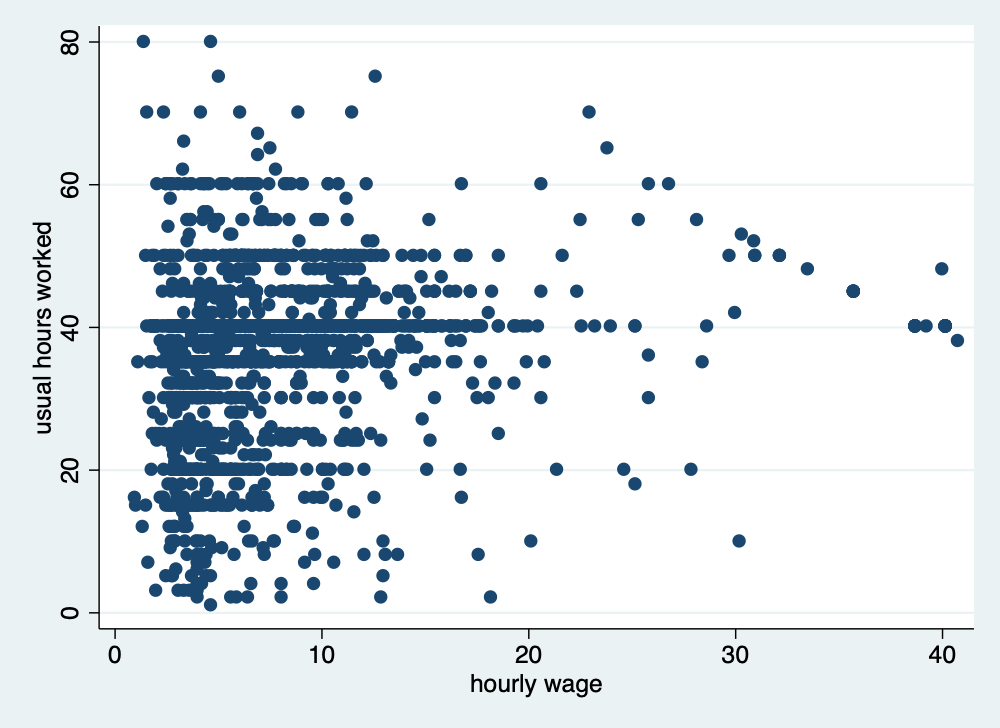
\includegraphics[keepaspectratio]{hour_wage.png}}
\caption{Hours and Wages}
\end{figure}

\section{Fixing and correcting errors in data}\label{fixing-and-correcting-errors-in-data}

Let go ahead and fix some of these errors that we have found. A word of caution is that you may need to talk to the data stewards about the best ways to correct the data. You don't want to attempt to fix the measurement error and introduce additional problems. Institutional knowledge of the data is very helpful before correcting errors.

Let's fix when race was equal to 4 when there are only 3 categories. Let's add a note for future users, which is good practice for replication.

\begin{Shaded}
\begin{Highlighting}[]
\KeywordTok{quietly}\NormalTok{ cd }\StringTok{"/Users/Sam/Desktop/Econ 645/Data/Mitchell"}
\KeywordTok{quietly} \KeywordTok{use}\NormalTok{ wws, }\KeywordTok{clear}
\OtherTok{list}\NormalTok{ idcode race }\KeywordTok{if}\NormalTok{ race==4}
\KeywordTok{replace}\NormalTok{ race=1 }\KeywordTok{if}\NormalTok{ idcode == 543}
\KeywordTok{note}\NormalTok{ race: race changed to 1 (from 4) }\KeywordTok{for}\NormalTok{ idcode 543}
\KeywordTok{tabulate}\NormalTok{ race}
\end{Highlighting}
\end{Shaded}

\begin{verbatim}
      | idcode   race |
      |---------------|
2013. |    543      4 |
      +---------------+

(1 real change made)

       race |      Freq.     Percent        Cum.
------------+-----------------------------------
          1 |      1,637       72.89       72.89
          2 |        583       25.96       98.84
          3 |         26        1.16      100.00
------------+-----------------------------------
      Total |      2,246      100.00
\end{verbatim}

Let's fix college gradudate when there were only 8 years of education.

\begin{Shaded}
\begin{Highlighting}[]
\KeywordTok{quietly}\NormalTok{ cd }\StringTok{"/Users/Sam/Desktop/Econ 645/Data/Mitchell"}
\KeywordTok{quietly} \KeywordTok{use}\NormalTok{ wws, }\KeywordTok{clear}
\OtherTok{list}\NormalTok{ idcode collgrad }\KeywordTok{if}\NormalTok{ yrschool \textless{} 12 \& collgrad == 1}
\KeywordTok{replace}\NormalTok{ collgrad = 0 }\KeywordTok{if}\NormalTok{ idcode == 107}

\KeywordTok{note}\NormalTok{ collgrad: collgrad changed to 0 (from 1) }\KeywordTok{for}\NormalTok{ idcode 107}
\KeywordTok{tab}\NormalTok{ yrschool collgrad}
\end{Highlighting}
\end{Shaded}

\begin{verbatim}
      | idcode   collgrad |
      |-------------------|
2198. |    107          1 |
      +-------------------+

(1 real change made)



  Years of |
    school |   college graduate
 completed |         0          1 |     Total
-----------+----------------------+----------
         8 |        70          0 |        70 
         9 |        55          0 |        55 
        10 |        84          0 |        84 
        11 |       123          0 |       123 
        12 |       943          0 |       943 
        13 |       174          2 |       176 
        14 |       180          7 |       187 
        15 |        81         11 |        92 
        16 |         0        252 |       252 
        17 |         0        106 |       106 
        18 |         0        154 |       154 
-----------+----------------------+----------
     Total |     1,710        532 |     2,242 
\end{verbatim}

Let's fix age which where the digits were switched, and we will make a note of it.

\begin{Shaded}
\begin{Highlighting}[]
\KeywordTok{quietly}\NormalTok{ cd }\StringTok{"/Users/Sam/Desktop/Econ 645/Data/Mitchell"}
\KeywordTok{quietly} \KeywordTok{use}\NormalTok{ wws, }\KeywordTok{clear}
\OtherTok{list}\NormalTok{ idcode age }\KeywordTok{if}\NormalTok{ age \textgreater{} 50}
\KeywordTok{replace}\NormalTok{ age = 38 }\KeywordTok{if}\NormalTok{ idcode == 51}
\KeywordTok{replace}\NormalTok{ age = 45 }\KeywordTok{if}\NormalTok{ idcode == 80}
\KeywordTok{note}\NormalTok{ age: the }\OtherTok{value} \KeywordTok{of}\NormalTok{ 83 was corrected to 38 }\KeywordTok{for}\NormalTok{ idcode 51}
\KeywordTok{note}\NormalTok{ age: the }\OtherTok{value} \KeywordTok{of}\NormalTok{ 54 was corrected to 45 }\KeywordTok{for}\NormalTok{ idcode 80}
\KeywordTok{tab}\NormalTok{ age}
\end{Highlighting}
\end{Shaded}

\begin{verbatim}
      | idcode   age |
      |--------------|
2205. |     80    54 |
2219. |     51    83 |
      +--------------+

(1 real change made)

(1 real change made)

     age in |
    current |
       year |      Freq.     Percent        Cum.
------------+-----------------------------------
         21 |          2        0.09        0.09
         22 |          8        0.36        0.45
         23 |         16        0.71        1.16
         24 |         35        1.56        2.72
         25 |         44        1.96        4.67
         26 |         50        2.23        6.90
         27 |         50        2.23        9.13
         28 |         63        2.80       11.93
         29 |         49        2.18       14.11
         30 |         55        2.45       16.56
         31 |         57        2.54       19.10
         32 |         60        2.67       21.77
         33 |         56        2.49       24.27
         34 |         95        4.23       28.50
         35 |        213        9.48       37.98
         36 |        224        9.97       47.95
         37 |        171        7.61       55.57
         38 |        176        7.84       63.40
         39 |        167        7.44       70.84
         40 |        139        6.19       77.03
         41 |        148        6.59       83.62
         42 |        111        4.94       88.56
         43 |        110        4.90       93.46
         44 |         98        4.36       97.82
         45 |         46        2.05       99.87
         46 |          1        0.04       99.91
         47 |          1        0.04       99.96
         48 |          1        0.04      100.00
------------+-----------------------------------
      Total |      2,246      100.00
\end{verbatim}

Let's look at our notes with the \emph{note} command.

\begin{Shaded}
\begin{Highlighting}[]
\KeywordTok{note}
\end{Highlighting}
\end{Shaded}

\begin{verbatim}
_dta:
  1.  This is a hypothetical dataset and should not be used for analysis purposes

age:
  1.  the value of 83 was corrected to 38 for idcode 51
  2.  the value of 54 was corrected to 45 for idcode 80

race:
  1.  race changed to 1 (from 4) for idcode 543

collgrad:
  1.  collgrad changed to 0 (from 1) for idcode 107
\end{verbatim}

\section{Identifying duplicates}\label{identifying-duplicates}

The duplicates command can be helpful, but it will only find duplicates that are exactly the same \textbf{unless you specify which variables with duplicates list vars}.
We'll cover this a bit later.

We need to be careful with duplicate observations. When working with panel data we will want multiple observations of the same cross-sectional unit, but there should be multiple observations for different time units and not the same time unit.

We can start with our \emph{duplicates} list command to find rows that are completely the same. This command will show all the duplicates. \textbf{Note:} for duplicate records to be found, all data needs to be the same.

\begin{Shaded}
\begin{Highlighting}[]
\KeywordTok{quietly}\NormalTok{ cd }\StringTok{"/Users/Sam/Desktop/Econ 645/Data/Mitchell"}
\KeywordTok{quietly} \KeywordTok{use} \StringTok{"dentists\_dups.dta"}\NormalTok{, }\KeywordTok{clear}
\KeywordTok{duplicates} \OtherTok{list}
\end{Highlighting}
\end{Shaded}

\begin{verbatim}
Duplicates in terms of all variables

  +-----------------------------------------------------------+
  | group:   obs:             name   years   fulltime   recom |
  |-----------------------------------------------------------|
  |      1      4       Mike Avity     8.5          0       0 |
  |      1      6       Mike Avity     8.5          0       0 |
  |      1      8       Mike Avity     8.5          0       0 |
  |      2      1   Olive Tu'Drill   10.25          1       1 |
  |      2     11   Olive Tu'Drill   10.25          1       1 |
  |-----------------------------------------------------------|
  |      3      2     Ruth Canaale      22          1       1 |
  |      3      3     Ruth Canaale      22          1       1 |
  +-----------------------------------------------------------+
\end{verbatim}

We'll have a more condensed version with duplicates examples. It will give an
example of the duplicate records for each group of duplicate records.

\begin{Shaded}
\begin{Highlighting}[]
\KeywordTok{duplicates}\NormalTok{ examples }
\end{Highlighting}
\end{Shaded}

\begin{verbatim}
Duplicates in terms of all variables

  +-------------------------------------------------------------------+
  | group:   #   e.g. obs             name   years   fulltime   recom |
  |-------------------------------------------------------------------|
  |      1   3          4       Mike Avity     8.5          0       0 |
  |      2   2          1   Olive Tu'Drill   10.25          1       1 |
  |      3   2          2     Ruth Canaale      22          1       1 |
  +-------------------------------------------------------------------+
\end{verbatim}

We can find the a consice list of duplicate records with duplicates report.

\begin{Shaded}
\begin{Highlighting}[]
\KeywordTok{duplicates} \KeywordTok{report}
\end{Highlighting}
\end{Shaded}

\begin{verbatim}
Duplicates in terms of all variables

--------------------------------------
   copies | observations       surplus
----------+---------------------------
        1 |            4             0
        2 |            4             2
        3 |            3             2
--------------------------------------
\end{verbatim}

The duplicates tag command can return the number of duplicates for each group of duplicates (note the separator option puts a line in the table after \# rows.

\begin{Shaded}
\begin{Highlighting}[]
\KeywordTok{duplicates} \FunctionTok{tag}\NormalTok{, }\KeywordTok{generate}\NormalTok{(dup)}
\OtherTok{list}\NormalTok{, separator(2)}
\end{Highlighting}
\end{Shaded}

\begin{verbatim}
Duplicates in terms of all variables

     +----------------------------------------------------+
     |              name   years   fulltime   recom   dup |
     |----------------------------------------------------|
  1. |    Olive Tu'Drill   10.25          1       1     1 |
  2. |      Ruth Canaale      22          1       1     1 |
     |----------------------------------------------------|
  3. |      Ruth Canaale      22          1       1     1 |
  4. |        Mike Avity     8.5          0       0     2 |
     |----------------------------------------------------|
  5. |        Mary Smith       3          1       1     0 |
  6. |        Mike Avity     8.5          0       0     2 |
     |----------------------------------------------------|
  7. | Y. Don Uflossmore    7.25          0       1     0 |
  8. |        Mike Avity     8.5          0       0     2 |
     |----------------------------------------------------|
  9. |        Mary Smith      27          0       0     0 |
 10. | Isaac O'Yerbreath   32.75          1       1     0 |
     |----------------------------------------------------|
 11. |    Olive Tu'Drill   10.25          1       1     1 |
     +----------------------------------------------------+
\end{verbatim}

Let's sort our data for better legibility, and then we will add lines in our output table whenever there is a new group.

\begin{Shaded}
\begin{Highlighting}[]
\KeywordTok{quietly}\NormalTok{ cd }\StringTok{"/Users/Sam/Desktop/Econ 645/Data/Mitchell"}
\KeywordTok{quietly} \KeywordTok{use} \StringTok{"dentists\_dups.dta"}\NormalTok{, }\KeywordTok{clear}
\KeywordTok{sort} \BaseNTok{name}\NormalTok{ years}
\OtherTok{list}\NormalTok{, sepby(}\BaseNTok{name}\NormalTok{ years)}
\end{Highlighting}
\end{Shaded}

\begin{verbatim}
     |              name   years   fulltime   recom |
     |----------------------------------------------|
  1. | Isaac O'Yerbreath   32.75          1       1 |
     |----------------------------------------------|
  2. |        Mary Smith       3          1       1 |
     |----------------------------------------------|
  3. |        Mary Smith      27          0       0 |
     |----------------------------------------------|
  4. |        Mike Avity     8.5          0       0 |
  5. |        Mike Avity     8.5          0       0 |
  6. |        Mike Avity     8.5          0       0 |
     |----------------------------------------------|
  7. |    Olive Tu'Drill   10.25          1       1 |
  8. |    Olive Tu'Drill   10.25          1       1 |
     |----------------------------------------------|
  9. |      Ruth Canaale      22          1       1 |
 10. |      Ruth Canaale      22          1       1 |
     |----------------------------------------------|
 11. | Y. Don Uflossmore    7.25          0       1 |
     +----------------------------------------------+
\end{verbatim}

\textbf{Notice!} There are two observations for Mary Smith, but one has 3 years of experience and the other one has 27 years, so it does not appear as a duplicate.

If there were too many variables, which could use our data browser.

\begin{Shaded}
\begin{Highlighting}[]
\NormalTok{browse }\KeywordTok{if}\NormalTok{ dup \textgreater{} 0}
\end{Highlighting}
\end{Shaded}

We will want to drop our duplicates, but not the first observation. The duplicates drop command will drop the duplicate records but still keep one observation of the duplicate group.

\begin{Shaded}
\begin{Highlighting}[]
\KeywordTok{duplicates} \KeywordTok{drop}
\end{Highlighting}
\end{Shaded}

Let's use a new dataset that is a bit more practical

\begin{verbatim}
use "wws.dta", replace
\end{verbatim}

Let's check for duplicate idcodes with the \emph{isid command}. If there is a duplicate idcode, the command will return an error.

\begin{Shaded}
\begin{Highlighting}[]
\KeywordTok{quietly}\NormalTok{ cd }\StringTok{"/Users/Sam/Desktop/Econ 645/Data/Mitchell"}
\KeywordTok{use} \StringTok{"wws.dta"}\NormalTok{, }\KeywordTok{replace}
\KeywordTok{isid}\NormalTok{ idcode}
\end{Highlighting}
\end{Shaded}

\begin{verbatim}
(Working Women Survey)
\end{verbatim}

Or just use duplicates list for the variable of interest

\begin{Shaded}
\begin{Highlighting}[]
\KeywordTok{quietly}\NormalTok{ cd }\StringTok{"/Users/Sam/Desktop/Econ 645/Data/Mitchell"}
\KeywordTok{quietly} \KeywordTok{use} \StringTok{"wws.dta"}\NormalTok{, }\KeywordTok{replace}
\KeywordTok{duplicates} \OtherTok{list}\NormalTok{ idcode}
\end{Highlighting}
\end{Shaded}

\begin{verbatim}
Duplicates in terms of idcode

(0 observations are duplicates)
\end{verbatim}

There are no duplicate idcodes, so we should expect that duplicates list will not return any duplicates, since every single values needs to be the same for there to be a dupicate record.

Let's use a dataset that does have duplicates. Let's check for duplicate idcodes.

\begin{Shaded}
\begin{Highlighting}[]
\KeywordTok{quietly}\NormalTok{ cd }\StringTok{"/Users/Sam/Desktop/Econ 645/Data/Mitchell"}
\KeywordTok{use} \StringTok{"wws\_dups.dta"}\NormalTok{, }\KeywordTok{clear}
\KeywordTok{isid}\NormalTok{ idcode}
\end{Highlighting}
\end{Shaded}

\begin{verbatim}
variable idcode does not uniquely identify the observations
r(459);

r(459);
\end{verbatim}

Or

\begin{Shaded}
\begin{Highlighting}[]
\KeywordTok{quietly}\NormalTok{ cd }\StringTok{"/Users/Sam/Desktop/Econ 645/Data/Mitchell"}
\KeywordTok{use} \StringTok{"wws\_dups.dta"}\NormalTok{, }\KeywordTok{clear}
\KeywordTok{duplicates} \OtherTok{list}\NormalTok{ idcode, sepby(idcode)}
\end{Highlighting}
\end{Shaded}

\begin{verbatim}
Duplicates in terms of idcode

  +------------------------+
  | group:   obs:   idcode |
  |------------------------|
  |      1   1088     2831 |
  |      1   2248     2831 |
  |------------------------|
  |      2   1244     3905 |
  |      2   1245     3905 |
  |------------------------|
  |      3    277     4214 |
  |      3   2247     4214 |
  +------------------------+
\end{verbatim}

I prefer \emph{duplicates list var1}, since an error will break the do file.

Let's generate our dup variable for identifying the number of duplicates per
group of duplicates.

\begin{Shaded}
\begin{Highlighting}[]
\KeywordTok{duplicates} \FunctionTok{tag}\NormalTok{ idcode, }\KeywordTok{generate}\NormalTok{(iddup)}
\end{Highlighting}
\end{Shaded}

Let's generate a different duplicate variable to find complete duplicate
records. Notice that we do not specify a variable after tag.

\begin{Shaded}
\begin{Highlighting}[]
\KeywordTok{duplicates} \FunctionTok{tag}\NormalTok{, }\KeywordTok{generate}\NormalTok{(alldup)}
\end{Highlighting}
\end{Shaded}

Let's list the data

\begin{Shaded}
\begin{Highlighting}[]
\OtherTok{list}\NormalTok{ idcode age race yrschool occupation wage }\KeywordTok{if}\NormalTok{ iddup==1 \& alldup==0}
\end{Highlighting}
\end{Shaded}

\begin{verbatim}
Duplicates in terms of idcode


Duplicates in terms of all variables

      +------------------------------------------------------+
      | idcode   age   race   yrschool   occupa~n       wage |
      |------------------------------------------------------|
1244. |   3905    36      1         14         11   4.339774 |
1245. |   3905    41      1         10          5   7.004828 |
      +------------------------------------------------------+
\end{verbatim}

It seems that idcode 3905 is a different person with a possible incorrect idcode. Let's fix that.

\begin{Shaded}
\begin{Highlighting}[]
\KeywordTok{replace}\NormalTok{ idcode=5160 }\KeywordTok{if}\NormalTok{ idcode==3905 \& age==41}
\OtherTok{list}\NormalTok{ idcode age race yrschool occupation wage }\KeywordTok{if}\NormalTok{ iddup==1 \& alldup==0}
\end{Highlighting}
\end{Shaded}

\begin{verbatim}
(1 real change made)

      +------------------------------------------------------+
      | idcode   age   race   yrschool   occupa~n       wage |
      |------------------------------------------------------|
1244. |   3905    36      1         14         11   4.339774 |
1245. |   5160    41      1         10          5   7.004828 |
      +------------------------------------------------------+
\end{verbatim}

Let's look observation that are complete duplicates.

\begin{Shaded}
\begin{Highlighting}[]
\KeywordTok{duplicates} \KeywordTok{report}
\OtherTok{list}\NormalTok{ idcode age race yrschool occupation wage }\KeywordTok{if}\NormalTok{ iddup==1 \& alldup==1}
\end{Highlighting}
\end{Shaded}

\begin{verbatim}
Duplicates in terms of all variables

--------------------------------------
   copies | observations       surplus
----------+---------------------------
        1 |         2244             0
        2 |            4             2
--------------------------------------

      +------------------------------------------------------+
      | idcode   age   race   yrschool   occupa~n       wage |
      |------------------------------------------------------|
 277. |   4214    35      1         17         13   11.27214 |
1088. |   2831    37      2          8          8   2.697261 |
2247. |   4214    35      1         17         13   11.27214 |
2248. |   2831    37      2          8          8   2.697261 |
      +------------------------------------------------------+
\end{verbatim}

We need to keep 1 observation of the duplicates. Use the \emph{duplicates drop} command.

\begin{Shaded}
\begin{Highlighting}[]
\KeywordTok{duplicates} \KeywordTok{drop}
\KeywordTok{duplicates} \KeywordTok{report}
\end{Highlighting}
\end{Shaded}

\begin{verbatim}
Duplicates in terms of all variables

(2 observations deleted)


Duplicates in terms of all variables

--------------------------------------
   copies | observations       surplus
----------+---------------------------
        1 |         2246             0
--------------------------------------
\end{verbatim}

\section{Practice}\label{practice}

Let's work the Census CPS.

Pull the Census CPS.
- You can download the file and import it, or
- You can use Stata to pull the file.

\begin{Shaded}
\begin{Highlighting}[]
\NormalTok{import delimited }\KeywordTok{using} \StringTok{"https://www2.census.gov/programs{-}surveys/cps/datasets/2025/basic/jul25pub.csv"}\NormalTok{, }\KeywordTok{clear}
\end{Highlighting}
\end{Shaded}

Let's save a copy of the csv file in Stata

Let's grab the data dictionary. Hint search: ``Census CPS 2025 data dictionary''

Let's check our data.
- What variable contains our laborforce status?
- What variable contains our weekly earnings?
- Does everyone employed have weekly earnings? Hint: Try \emph{summarize}
- What flag with our weekly earning that provides information about available data?
- Try \emph{tabstat} with the flag and weekly earnings. What do you find?
- Try \emph{tabstat} with statistics(n mean sd p25 p50 p75)
- What are our identifier variable(s)? How many did you find?
- Are there any duplicate records?

Mitchell, N.M. (2020). \emph{Data Management Using Stata: A Practical Handbook}. (2nd ed.). Stata Press.

UCLA Advanced Research Computing. (2025). \emph{Stata Learning Modules.} Retrieved from \url{https://stats.oarc.ucla.edu/stata/modules/}

\bibliography{book.bib,packages.bib}

\end{document}
